% Content fragment for Overleaf. Requires \usepackage{longtable,graphicx,float,svg}.
\section{System Analysis}
\label{sec:sys-analysis}
\subsection{Stakeholders}

BK Uni's stakeholders include Students and Administrators. Students use the system to track their progress and plan their studies; Administrators maintain curriculum data and academic rules. Academic advisors understand Students' curricula but do not operate BK Uni.

\subsubsection{Students}
Students are BK Uni's primary users and direct beneficiaries. They need to track their academic progress, understand curriculum requirements, and prepare plans for upcoming semesters.

\textbf{Needs and goals:}
\begin{itemize}
    \item Review courses that can count toward completing a curriculum (required courses, major elective groups, and free electives), together with the relationships and constraints governing course registration, selection, and completion (including, but not limited to, prerequisites and credit requirements where applicable).
    \item Record the academic status of each course and its planned semester to keep their personal progress up to date.
    \item Identify outstanding required courses, elective requirements, or educational regulations, and check eligibility for subsequent courses.
    \item Receive course recommendations for a planned semester, with explanations of recommended and deferred courses and applicable credit limits.
\end{itemize}

\textbf{Roles and responsibilities:}
\begin{itemize}
    \item Create and manage a personal profile and select the correct curriculum.
    \item Accurately update the status of their courses.
    \item Check their input data and compare recommendations with official university information before making enrollment decisions.
\end{itemize}

BK Uni helps Students plan their studies and understand rules based on the available data. Its results do not confirm official enrollment eligibility or replace academic advising.

\subsubsection{Administrators}
Administrators maintain the foundational data BK Uni uses to analyze academic progress and generate course recommendations. The accuracy, completeness, and consistency of this data directly affect the quality of results for Students.

\textbf{Needs and goals:}
\begin{itemize}
    \item Manage the course catalog and curricula together with related data such as curriculum courses, recommended semesters, and elective groups.
    \item Define and update academic rules, including prerequisites and minimum credit requirements.
    \item Ensure data and rules are associated with the correct curriculum and do not affect other curricula.
    \item Maintain sufficiently clear data so that analyses and recommendations can be explained.
\end{itemize}

\textbf{Roles and responsibilities:}
\begin{itemize}
    \item Create, edit, and manage course and curriculum data within the scope of their administrative permissions.
    \item Check the accuracy and consistency of curriculum data.
    \item Update data when changes occur and make clear that results depend on the available data.
\end{itemize}

Administrators manage data in BK Uni but do not replace academic units in issuing or confirming official academic regulations.

\subsubsection{Academic Advisors}
Academic advisors help Students make informed decisions and review study plans against official curriculum regulations. They are indirect stakeholders: they do not sign in to, access, or operate BK Uni; advising takes place outside the system. When Students consult them in person, advisors need clear information about the Students' progress, outstanding academic requirements, and proposed plans.

\textbf{Stakeholder summary:}
\begin{longtable}{|p{0.20\textwidth}|p{0.28\textwidth}|p{0.42\textwidth}|}
\hline
\textbf{Stakeholder} & \textbf{Involvement} & \textbf{Primary concern} \\
\hline
\endfirsthead
\hline
\textbf{Stakeholder} & \textbf{Involvement} & \textbf{Primary concern} \\
\hline
\endhead
Student & Direct, primary user & Tracking progress, checking eligibility, and planning semesters \\
\hline
Administrator & Direct, data manager & Maintaining the course catalog, curricula, and course rules \\
\hline
Academic advisor & Indirect, does not operate the system & Helping Students review plans against official regulations \\
\hline
\end{longtable}

\subsection{Actors \& Roles}

An actor is an individual, group, or external system that interacts with BK Uni. A role defines the scope of functions and data each actor is permitted to use. The system's actors are Student and Admin.

\subsubsection{Student}
Students are users signed in with student accounts and are the primary actors using BK Uni's study-planning functions.

\textbf{Roles and permissions:}
\begin{itemize}
    \item Create and update their own academic profiles and select a curriculum.
    \item Record course statuses, planned semesters, and the status of educational regulations, and view their personal progress.
    \item Analyze course eligibility, review outstanding requirements, and receive explained semester recommendations.
    \item View or modify only profiles and personal data they own; they cannot modify standard curriculum data.
\end{itemize}

\subsubsection{Admin}
Admins are responsible for managing course data, curricula, and the academic rules used by the system.

\textbf{Roles and permissions:}
\begin{itemize}
    \item Manage the course catalog and the list of semesters in which each course has been offered.
    \item Create, update, and manage standard curricula.
    \item Manage curriculum courses, recommended semesters, elective groups, course rules, and educational regulations.
    \item View the course catalog and course details in the same way as Students.
    \item Ensure data is associated with the correct curriculum and is sufficiently accurate for analysis.
    \item They cannot access Students' personal profiles or study plans.
\end{itemize}

Admin privileges are granted under controlled authorization so that only people responsible for administration can modify standard data.

\textbf{Access-control summary:}
\begin{longtable}{|p{0.16\textwidth}|p{0.36\textwidth}|p{0.38\textwidth}|}
\hline
\textbf{Actor} & \textbf{Access} & \textbf{Primary permissions} \\
\hline
\endfirsthead
\hline
\textbf{Actor} & \textbf{Access} & \textbf{Primary permissions} \\
\hline
\endhead
Student & Their own profile and academic data & Manage profile, update progress, view analyses, and plan studies \\
\hline
Admin & Course data and standard curriculum data & Manage courses, curricula, recommended semesters, elective groups, rules, and regulations; view the course catalog \\
\hline
\end{longtable}

\subsection{Functional Requirements}

Functional requirements describe the services BK Uni must provide to its actors. Each requirement is expressed as desired system behavior and can serve as a basis for design, use-case development, and acceptance testing.

\subsubsection{FR-1. Accounts and Access}
\begin{longtable}{|p{0.10\textwidth}|p{0.15\textwidth}|p{0.65\textwidth}|}
\hline
\textbf{ID} & \textbf{Role} & \textbf{Requirement} \\
\hline
\endfirsthead
\hline
\textbf{ID} & \textbf{Role} & \textbf{Requirement} \\
\hline
\endhead
FR-1.1 & User / System & The system allows users to create an account using an email address and password; new accounts are assigned the Student role. \\
\hline
FR-1.2 & User & The system allows users to sign in to and sign out of their accounts. \\
\hline
FR-1.3 & System & The system allows only authenticated users to access functions and data that require an account. \\
\hline
FR-1.4 & System & The system restricts access according to role and data ownership; Students may only view or modify their own personal data, which the server identifies from the signed-in account rather than from identifiers sent by the client. \\
\hline
FR-1.5 & Admin / System & The system grants Admin privileges only to authorized accounts; Admin accounts are created by the system operator, cannot be registered through the user interface, and users cannot elevate their own privileges. \\
\hline
\end{longtable}

\subsubsection{FR-2. Student Profiles and Academic Progress}
\begin{longtable}{|p{0.10\textwidth}|p{0.15\textwidth}|p{0.65\textwidth}|}
\hline
\textbf{ID} & \textbf{Role} & \textbf{Requirement} \\
\hline
\endfirsthead
\hline
\textbf{ID} & \textbf{Role} & \textbf{Requirement} \\
\hline
\endhead
FR-2.1 & Student & A Student can create, view, and update their personal academic profile. \\
\hline
FR-2.2 & Student & A Student can select an appropriate curriculum from the list of available curricula. \\
\hline
FR-2.3 & Student & A Student can view, search, and filter the courses in their selected curriculum or in the entire course catalog. \\
\hline
FR-2.4 & Student & A Student can record each course's status as not started, in progress, completed, or failed. Changes are kept as a draft and saved together in one operation; unsaved changes can be discarded. \\
\hline
FR-2.5 & System & The system displays academic progress based on the selected curriculum and the course statuses provided by the Student. \\
\hline
FR-2.6 & Student & A Student can view the details of a course, including its general information, syllabus, and the semesters in which it has been offered. \\
\hline
FR-2.7 & Student / System & Graduation conditions that are not regular courses, such as the English-language graduation standard or the physical-education certificate, are loaded from the graduation-conditions section of the imported myBK report (FR-2.8) together with the course statuses; the Student does not mark them on a separate page. When a recommended roadmap schedules the graduation thesis while a required condition is not yet met, the system shows a reminder at that semester, and the Student can confirm there that the condition has been met; the confirmation is saved to the Student's progress. \\
\hline
FR-2.8 & Student / System & A Student can import their academic progress from the university's myBK progress report, either as a PDF file or as pasted text. Before anything is saved, the system shows a review that compares the report with the curriculum data and lists unknown course codes and differences. After the Student confirms, the system replaces the Student's course statuses with those in the report and stores the imported progress; the original file is not stored. \\
\hline
FR-2.9 & Student & After importing, a Student can adjust the imported progress, such as adding a note to a course or choosing which elective group a completed course counts toward. \\
\hline
\end{longtable}

\subsubsection{FR-3. Admin Course and Curriculum Management}
\begin{longtable}{|p{0.10\textwidth}|p{0.15\textwidth}|p{0.65\textwidth}|}
\hline
\textbf{ID} & \textbf{Role} & \textbf{Requirement} \\
\hline
\endfirsthead
\hline
\textbf{ID} & \textbf{Role} & \textbf{Requirement} \\
\hline
\endhead
FR-3.1 & Admin & An Admin can create, view, update, and delete curricula, including each curriculum's minimum and maximum credits per semester. \\
\hline
FR-3.2 & Admin & An Admin can add, edit, and delete courses in the course catalog, and add courses to or remove courses from a curriculum. \\
\hline
FR-3.3 & Admin & An Admin can manage the courses of each semester in a curriculum by setting a recommended academic year and semester for each course, and can manage credits and course classification (course categories). \\
\hline
FR-3.4 & Admin & An Admin can create and manage elective groups, their member courses, and each group's completion requirement (a number of courses or a number of credits). \\
\hline
FR-3.5 & Admin & An Admin can define, update, and remove relations between courses of a curriculum. Four relation types are supported: prerequisite (the related course must be passed), prior course (the related course must have been taken, even if failed), corequisite (the related course must be taken earlier or in the same semester), and recommended (advisory only). \\
\hline
FR-3.6 & System & The system associates courses and rules with the correct curriculum so that data for different curricula is managed independently. \\
\hline
FR-3.7 & Admin & An Admin can add, edit, and delete educational and academic regulations. These are curriculum-related requirements that are not specific to individual courses, such as English-language certification, computer-skills certification, or social-work requirements. \\
\hline
FR-3.8 & Admin & An Admin can manage the list of semesters in which each course has been offered. The system uses this history to estimate whether a course is likely to be offered in a future semester; the estimate produces warnings and preferences, not hard rules. \\
\hline
FR-3.9 & System & The system stores the specializations of each curriculum and the elective groups that belong to each specialization. This data is loaded together with the curriculum and can be maintained through the administration API. \\
\hline
FR-3.10 & Admin & An Admin can import course syllabi from a structured file through the administration API. An import only adds or updates syllabi, identified by course code and version, and never deletes syllabi or changes courses and course relations. \\
\hline
FR-3.11 & System & The system operator can load the structure of a curriculum (courses, recommended semesters, elective groups, and relations) from the university's published curriculum data instead of entering it by hand. \\
\hline
\end{longtable}

\subsubsection{FR-4. Eligibility and Curriculum Requirement Analysis}
\begin{longtable}{|p{0.10\textwidth}|p{0.15\textwidth}|p{0.65\textwidth}|}
\hline
\textbf{ID} & \textbf{Role} & \textbf{Requirement} \\
\hline
\endfirsthead
\hline
\textbf{ID} & \textbf{Role} & \textbf{Requirement} \\
\hline
\endhead
FR-4.1 & Student & A Student can view an analysis of their progress and course eligibility based on their personal profile and selected curriculum. \\
\hline
FR-4.2 & System & The system determines whether the Student is eligible to take a course, based on data entered by Admins (courses, course relations, and curriculum rules) and data entered by the Student (courses completed, in progress, and failed). \\
\hline
FR-4.3 & System & The system identifies the courses, elective-group requirements, and educational regulations that the Student still needs to complete. \\
\hline
FR-4.4 & System & The system explains its results by identifying relevant conditions, such as an uncompleted prerequisite or an unmet credit requirement. \\
\hline
FR-4.5 & System & Analysis results are recomputed from current data each time the Student views them, so they always reflect the latest academic status and curriculum data; the system does not store a history of analyses. \\
\hline
\end{longtable}

\subsubsection{FR-5. Course Recommendations}
\begin{longtable}{|p{0.10\textwidth}|p{0.15\textwidth}|p{0.65\textwidth}|}
\hline
\textbf{ID} & \textbf{Role} & \textbf{Requirement} \\
\hline
\endfirsthead
\hline
\textbf{ID} & \textbf{Role} & \textbf{Requirement} \\
\hline
\endhead
FR-5.1 & Student & A Student can request a recommended study roadmap. The system computes a roadmap only when the Student explicitly requests it; changing settings alone does not start a computation. \\
\hline
FR-5.2 & System & The system builds the input for a roadmap from the selected curriculum, the Student's course statuses and imported progress, course relations, offering history, and the credit limits of each semester. \\
\hline
FR-5.3 & System & The system generates the roadmap with a constraint solver so that every hard constraint is satisfied: course relations, credit limits per semester, completion requirements of required courses and elective groups, and the settings the Student has fixed. Each recommended course comes with the reason it was placed in its semester. \\
\hline
FR-5.4 & System & The system does not make recommendations that conflict with curriculum constraints or the academic information provided by the Student; every generated roadmap is checked again against the curriculum rules, and any violation is reported. \\
\hline
FR-5.5 & System & The system presents the roadmap semester by semester with its courses, credits, the expected graduation semester, the assumptions used, and warnings, such as a course that has rarely been offered in the planned semester. \\
\hline
FR-5.6 & System & If no roadmap satisfies the constraints, the system reports this, identifies which of the Student's settings make the problem infeasible, and proposes fixes (for example, removing a pinned course or allowing a summer semester) that the Student can apply and solve again. The system never bypasses curriculum rules to produce a result. If the solver does not finish within its time limit, the system reports a timeout instead of an unverified result. \\
\hline
FR-5.7 & Student & A Student can view recommended courses for each semester from the next semester through graduation, rather than only for the next semester. \\
\hline
FR-5.8 & Student & A Student can state study preferences: a maximum or target number of credits for each semester, a graduation deadline, courses they want to take, the priority order of these goals, summer semesters they want to study, and semesters they will skip. \\
\hline
FR-5.9 & Student & A Student can pin a course to a specific semester, freeze a semester so that only its pinned courses are kept, and add a free-choice course by entering its course code; an unknown course code is rejected before solving. \\
\hline
FR-5.10 & Student & A Student can explore what-if scenarios: assume an in-progress course will be passed or failed, assume a planned course will be failed, or declare that a course is or is not offered in a given semester. \\
\hline
FR-5.11 & Student / System & A Student can save several named roadmaps and mark one as the baseline. When a new roadmap is generated, the system compares it with the baseline and shows the courses that moved, were added, or were removed. \\
\hline
FR-5.12 & System & The Student's settings and saved roadmaps are stored in their account and restored on the next sign-in. Saving them requires the Student to have imported their progress (FR-2.8). \\
\hline
FR-5.13 & System & A recommended roadmap is advisory only: generating it does not change the Student's course statuses, personal plan, or the curriculum, and it is not an official course registration. \\
\hline
FR-5.14 & System & Besides the default constraint solver used by the Student interface, the system provides an alternative answer-set programming engine through its API for comparison; this engine can also take the Student's interest tags into account. \\
\hline
\end{longtable}

\subsubsection{FR-6. Student Personal Plans}
\begin{longtable}{|p{0.10\textwidth}|p{0.15\textwidth}|p{0.65\textwidth}|}
\hline
\textbf{ID} & \textbf{Role} & \textbf{Requirement} \\
\hline
\endfirsthead
\hline
\textbf{ID} & \textbf{Role} & \textbf{Requirement} \\
\hline
\endhead
FR-6.1 & System & A personal plan assigns a planned semester to courses of a curriculum. Each Student has one personal plan for each curriculum, tied to their account; the plan shown is the one for the curriculum selected in the profile. \\
\hline
FR-6.2 & Student & A Student can add or remove courses from their personal plan and schedule courses in planned semesters without changing the standard curriculum. \\
\hline
FR-6.3 & Student / System & Course statuses, planned semesters, and notes entered by the Student are stored as the Student's own data, separate from the curriculum data managed by Admins; the Student's changes never modify the curriculum. \\
\hline
FR-6.4 & Student / System & When a course in the plan is changed, the system presents the course's current status and planned semester for the Student to review; changes are saved only when the Student confirms them. \\
\hline
FR-6.5 & System & When presenting personal-plan analysis results, the system must clearly distinguish content based on information provided by the Student (completed, in-progress, and planned courses) from content based on curriculum requirements. \\
\hline
FR-6.6 & System & If the course pathway declared by the Student does not satisfy curriculum requirements, the system reports each problem and its reason: a course planned before its prerequisites, a course planned in a semester that has already passed, a course that has not been offered in that term before, or a semester exceeding the maximum credits. \\
\hline
\end{longtable}

\subsection{Non-functional Requirements}

Non-functional requirements define BK Uni's quality and operational criteria. Quantitative criteria are evaluated in an agreed test environment using data representative of expected usage.

\subsubsection{NFR-1. Security}
\begin{longtable}{|p{0.12\textwidth}|p{0.78\textwidth}|}
\hline
\textbf{ID} & \textbf{Requirement} \\
\hline
\endfirsthead
\hline
\textbf{ID} & \textbf{Requirement} \\
\hline
\endhead
NFR-1.1 & The system must authenticate users before allowing access to private functions or data; authorization must be checked on the server for every request. \\
\hline
NFR-1.2 & Passwords must be stored as hashes using a dedicated password-hashing algorithm; plaintext passwords, session tokens, and system secrets must not be logged or returned to users. \\
\hline
NFR-1.3 & Login sessions must be protected using secure cookie mechanisms; data-changing operations must be protected against request forgery, and request origins must be validated. \\
\hline
NFR-1.4 & Data transmitted between clients and the server must be encrypted; database connection information and secret keys must be managed outside the source code. \\
\hline
NFR-1.5 & The system must reject invalid or unauthorized requests without disclosing another account's data or sensitive internal information. \\
\hline
\end{longtable}

\subsubsection{NFR-2. Performance}
\begin{longtable}{|p{0.12\textwidth}|p{0.78\textwidth}|}
\hline
\textbf{ID} & \textbf{Requirement} \\
\hline
\endfirsthead
\hline
\textbf{ID} & \textbf{Requirement} \\
\hline
\endhead
NFR-2.1 & Under expected usage load and with representative data, at least 95\% of routine operations (reading profiles, listing curricula, and updating statuses) must complete within 2 seconds. \\
\hline
NFR-2.2 & Under the same test conditions, at least 95\% of course analysis or recommendation requests must complete within 5 seconds. \\
\hline
NFR-2.3 & List pages must support appropriate search, filtering, or pagination so that response time does not increase linearly with the total number of records. \\
\hline
NFR-2.4 & Performance tests must record the 95th-percentile response time, error rate, and load configuration; results must be compared with the thresholds in NFR-2.1 and NFR-2.2. \\
\hline
\end{longtable}

\subsubsection{NFR-3. Reliability}
\begin{longtable}{|p{0.12\textwidth}|p{0.78\textwidth}|}
\hline
\textbf{ID} & \textbf{Requirement} \\
\hline
\endfirsthead
\hline
\textbf{ID} & \textbf{Requirement} \\
\hline
\endhead
NFR-3.1 & The system must achieve at least 95\% monthly availability, excluding scheduled maintenance announced in advance. \\
\hline
NFR-3.2 & A save operation must be atomic: if an error occurs partway through, the system must not leave data partially updated. \\
\hline
NFR-3.3 & Data must be backed up regularly; the recovery time objective (RTO) must not exceed 4 hours, and the recovery point objective (RPO) must not exceed 24 hours. \\
\hline
NFR-3.4 & When a dependent service fails, the system must clearly report that the operation was not completed and must not present a false success result or speculative data as an official result. \\
\hline
\end{longtable}

\subsubsection{NFR-4. Maintainability}
\begin{longtable}{|p{0.12\textwidth}|p{0.78\textwidth}|}
\hline
\textbf{ID} & \textbf{Requirement} \\
\hline
\endfirsthead
\hline
\textbf{ID} & \textbf{Requirement} \\
\hline
\endhead
NFR-4.1 & UI, business logic, authentication, and storage components must be organized by clearly defined responsibilities so that they can be changed independently where appropriate. \\
\hline
NFR-4.2 & Academic and business rules must be described consistently in design, implementation, and test documentation; changes to rules must be reflected in the relevant documentation. \\
\hline
NFR-4.3 & Core functions for access control, curriculum data, analysis, and recommendations must have automated tests covering valid, invalid, and important edge cases. \\
\hline
NFR-4.4 & Data structure changes must include migration instructions and error-handling procedures to prevent loss or corruption of existing data. \\
\hline
\end{longtable}

\subsubsection{NFR-5. Scalability}
\begin{longtable}{|p{0.12\textwidth}|p{0.78\textwidth}|}
\hline
\textbf{ID} & \textbf{Requirement} \\
\hline
\endfirsthead
\hline
\textbf{ID} & \textbf{Requirement} \\
\hline
\endhead
NFR-5.1 & The system must support growth in the number of users, curricula, courses, and academic data without changing the correctness of access control or business results. \\
\hline
NFR-5.2 & Queries for large data sets must be able to limit results through pagination or an equivalent mechanism; loading all data at once must not be required. \\
\hline
NFR-5.3 & Adding new types of academic rules or new features should not require rewriting unrelated authentication, profile, or administration flows. \\
\hline
NFR-5.4 & As load increases, processing capacity must be scalable by adding resources to appropriate components without requiring changes to the Student or Admin user interface. \\
\hline
\end{longtable}

\subsubsection{NFR-6. Usability}
\begin{longtable}{|p{0.12\textwidth}|p{0.78\textwidth}|}
\hline
\textbf{ID} & \textbf{Requirement} \\
\hline
\endfirsthead
\hline
\textbf{ID} & \textbf{Requirement} \\
\hline
\endhead
NFR-6.1 & The user interface, instructions, and user notifications must use clear and consistent Vietnamese; technical terms should be explained when necessary. \\
\hline
NFR-6.2 & Students must be able to complete the main flows---updating their profile, recording course statuses, viewing analysis, and generating recommendations---without technical knowledge. \\
\hline
NFR-6.3 & Every screen must clearly indicate loading, success, empty, and error states; notifications should explain the next steps where possible. \\
\hline
NFR-6.4 & Analysis results and recommendations must clearly present met and unmet conditions, outstanding requirements, total credits, and the reasons courses were recommended or deferred. \\
\hline
NFR-6.5 & Actions with significant effects on data, such as deletion or confirmation of plan changes, must clearly explain their consequences and require user confirmation. \\
\hline
NFR-6.6 & The interface must be usable on common desktop and mobile devices, with readable content, consistent navigation, and error messages associated with the relevant action. \\
\hline
NFR-6.7 & After signing in, Students must be able to open the system's main features (Academic Analysis and Course Recommendations) within no more than two navigation actions from the main menu. \\
\hline
\end{longtable}

\subsubsection{NFR-7. Auditability}
\begin{longtable}{|p{0.12\textwidth}|p{0.78\textwidth}|}
\hline
\textbf{ID} & \textbf{Requirement} \\
\hline
\endfirsthead
\hline
\textbf{ID} & \textbf{Requirement} \\
\hline
\endhead
NFR-7.1 & The system must record important changes to curricula, courses, elective groups, and rules, including the person responsible, time, affected item, and change details. \\
\hline
NFR-7.2 & The system must record account and access-related events, such as sign-ins, sign-outs, permission changes, and denied access attempts, to the extent necessary for investigation. \\
\hline
\end{longtable}

\subsection{Usecase Diagram}

The following use case diagrams illustrate the main interactions between Guests, Students, Admins, and BK Uni. The overview summarizes the system's scope; each of the following diagrams details one group of functional requirements. All diagrams use the same notation: a solid arrow links an actor to a use case it starts, a dashed arrow labeled \incl{} or \extd{} shows inclusion or extension, and a hollow triangle shows generalization.

\subsubsection{System Overview}
\begin{figure}[H]
    \centering
    \begin{tikzpicture}
  \ucactor{guest}{0,8.4}{Guest}
  \ucactor{student}{0,3.2}{Student}
  \ucactor{admin}{0,-3.6}{Admin}
  \ucactor{ai}{12.4,-0.6}{AI Service\\\scriptsize\guillemotleft system\guillemotright}

  \node[ucwide] (reg)  at (6.4,8.4)  {Register Account};
  \node[ucwide] (prof) at (6.4,6.9)  {Manage Profile and\\Course Progress};
  \node[ucwide] (mybk) at (6.4,5.4)  {Import myBK Progress};
  \node[ucwide] (plan) at (6.4,4.0)  {Manage Personal Plan};
  \node[ucwide] (ana)  at (6.4,2.6)  {View Progress and Analysis};
  \node[ucwide] (rec)  at (6.4,1.1)  {Get Study Roadmap\\Recommendations};
  \node[ucwide] (ai1)  at (6.4,-0.4) {AI Academic Advising};
  \node[ucwide] (acc)  at (6.4,-1.8) {Sign In / Sign Out};
  \node[ucwide] (cat)  at (6.4,-3.2) {Manage Course Catalog};
  \node[ucwide] (cur)  at (6.4,-4.6) {Manage Curricula};
  \coordinate (top) at (6.4,9.3);
  \ucsystem{(top)(reg)(cur)}{BK Uni}

  \draw[assoc] (guest) -- (reg.west);
  \foreach \u in {prof,mybk,plan,ana,rec,ai1,acc} \draw[assoc] (student) -- (\u.west);
  \foreach \u in {acc,cat,cur} \draw[assoc] (admin) -- (\u.west);
  \draw[assoc] (ai1.east) -- (ai);
\end{tikzpicture}

    \caption{BK Uni use case overview}
\end{figure}
Guests can only register an account. Students manage their profile and course progress, import their progress from myBK, edit a personal plan, view their progress analysis, and request study-roadmap recommendations. Admins maintain the course catalog and the curricula. Both Students and Admins sign in and sign out.

\subsubsection{Account and Access}
\begin{figure}[H]
    \centering
    \begin{tikzpicture}
  \ucactor{guest}{0,1.2}{Guest}
  \ucactor{student}{0,-1.6}{Student}
  \ucactor{admin}{0,-4.0}{Admin}

  \node[uc] (reg)  at (5.4,1.6)  {Register Account};
  \node[uc] (info) at (11.2,1.6) {Provide Email\\and Password};
  \node[uc] (in)   at (5.4,0.0)  {Sign In};
  \node[uc] (out)  at (5.4,-2.6) {Sign Out};
  \coordinate (top) at (5.4,2.5);
  \ucsystem{(top)(reg)(info)(out)}{Account and Access (FR-1)}

  \draw[assoc] (guest) -- (reg.west);
  \draw[assoc] (guest) -- (in.west);
  \draw[assoc] (student) -- (out.west);
  \draw[assoc] (admin) -- (out.west);
  \draw[inc] (reg) -- node[rel, above] {\incl} (info);

  \node[ucnote=9cm, anchor=north east] at ($(sysbox.south east)+(0,-0.25)$)
    {Registration creates Student accounts only. Admin accounts are created by the system operator (FR-1.5).};
\end{tikzpicture}

    \caption{Account and access use cases}
\end{figure}
Guests can register an account and sign in. Registration always includes providing an email address and a password and creates a Student account; Admin accounts are created by the system operator. Both Students and Admins can sign out.

\subsubsection{Student Profile and Progress}
\begin{figure}[H]
    \centering
    \begin{tikzpicture}
  \ucactor{student}{0,0.4}{Student}

  \node[uc] (prof)   at (5.6,5.4)  {Manage Profile};
  \node[uc] (cur)    at (5.6,3.6)  {Select Curriculum};
  \node[uc] (browse) at (5.6,2.0)  {Browse Courses};
  \node[uc] (detail) at (5.6,0.6)  {View Course Details};
  \node[uc] (status) at (5.6,-1.4) {Update Course Statuses};
  \node[uc] (mybk)   at (5.6,-4.4) {Import myBK Progress};

  \node[uc] (view)   at (11.8,6.0)  {View Profile};
  \node[uc] (upd)    at (11.8,4.7)  {Update Profile};
  \node[uc] (search) at (11.8,2.0)  {Search and\\Filter Courses};
  \node[uc] (draft)  at (11.8,-0.6) {Review and Save Draft};
  \node[uc] (file)   at (11.8,-2.1) {Import / Export Statuses\\(Excel or CSV)};
  \node[uc] (review) at (11.8,-3.7) {Review Report\\before Saving};
  \node[uc] (adj)    at (11.8,-5.2) {Adjust Imported\\Progress};
  \coordinate (top) at (5.6,6.9);
  \ucsystem{(top)(prof)(view)(adj)(mybk)}{Student Profile and Progress (FR-2)}

  \foreach \u in {prof,cur,browse,detail,status,mybk} \draw[assoc] (student) -- (\u.west);
  \draw[gen] (view.west) -- (prof);
  \draw[gen] (upd.west) -- (prof);
  \draw[inc] (search.west) -- node[rel, above] {\extd} (browse.east);
  \draw[inc] (status) -- node[rel, above, sloped] {\incl} (draft.west);
  \draw[inc] (file.west) -- node[rel, below, sloped] {\extd} (status);
  \draw[inc] (mybk) -- node[rel, above, sloped] {\incl} (review.west);
  \draw[inc] (adj.west) -- node[rel, below, sloped] {\extd} (mybk);

  \node[ucnote=9cm, anchor=north east] at ($(sysbox.south east)+(0,-0.25)$)
    {Importing replaces the course statuses and loads graduation conditions such as the English standard (FR-2.7, FR-2.8).};
\end{tikzpicture}

    \caption{Student profile and progress use cases}
\end{figure}
Students view and update their profile, select a curriculum, browse courses (optionally searching and filtering), and view course details. Course statuses are edited as a draft that is reviewed and saved in one operation; statuses can also be exported to and imported from an Excel or CSV file. Importing the myBK progress report always shows a review of the report before anything is saved, and the imported progress can be adjusted afterwards.

\subsubsection{Progress and Eligibility Analysis}
\begin{figure}[H]
    \centering
    \begin{tikzpicture}
  \ucactor{student}{0,0.6}{Student}

  \node[uc] (ana)  at (5.6,0.6)  {View Progress\\and Analysis};
  \node[uc] (cred) at (11.8,3.6)  {Compute Credit Progress\\by Knowledge Block};
  \node[uc] (elig) at (11.8,2.1)  {Check Course Eligibility};
  \node[uc] (miss) at (11.8,0.6)  {Identify Outstanding\\Requirements};
  \node[uc] (plan) at (11.8,-0.9) {Check Personal Plan};
  \node[uc] (expl) at (11.8,-2.4) {Explain Unmet\\Conditions};
  \coordinate (top) at (8,4.9);
  \ucsystem{(top)(ana)(cred)(expl)}{Progress and Eligibility Analysis (FR-4)}

  \draw[assoc] (student) -- (ana.west);
  \draw[inc] (ana) -- node[rel, above, sloped] {\incl} (cred.west);
  \draw[inc] (ana) -- node[rel, above, sloped] {\incl} (elig.west);
  \draw[inc] (ana) -- node[rel, above] {\incl} (miss.west);
  \draw[inc] (ana) -- node[rel, below, sloped] {\incl} (plan.west);
  \draw[inc] (expl.west) -- node[rel, below, sloped] {\extd} (ana);

  \node[ucnote=9cm, anchor=north east] at ($(sysbox.south east)+(0,-0.25)$)
    {Results are recomputed from current data every time they are viewed; no analysis history is stored (FR-4.5).};
\end{tikzpicture}

    \caption{Progress and eligibility analysis use cases}
\end{figure}
Viewing the analysis always computes credit progress by knowledge block, checks the eligibility of each course, identifies the courses, elective-group requirements, and regulations still outstanding, and checks the personal plan. The Student can additionally view why a condition is not met. The analysis is recomputed from current data each time and is never stored.

\subsubsection{Course Recommendations}
\begin{figure}[H]
    \centering
    \begin{tikzpicture}
  \ucactor{student}{0,0.2}{Student}

  \node[uc] (conf)  at (5.6,4.4)  {Configure Scenario};
  \node[uc] (solve) at (5.6,-0.4) {Solve Study Roadmap};
  \node[uc] (saved) at (5.6,-5.4) {Manage Saved Roadmaps};

  \node[uc] (pref)  at (11.8,7.0)  {Set Preferences};
  \node[uc] (pin)   at (11.8,5.7)  {Pin Course /\\Freeze Semester};
  \node[uc] (free)  at (11.8,4.2)  {Add Free-choice Course};
  \node[uc] (what)  at (11.8,2.9)  {Explore What-if\\Assumptions};
  \node[uc] (input) at (11.8,1.3)  {Build Input from\\Progress and Curriculum};
  \node[uc] (check) at (11.8,-0.2) {Verify Roadmap\\against Rules};
  \node[uc] (fail)  at (11.8,-1.7) {Report Infeasibility\\or Timeout};
  \node[uc] (fix)   at (11.8,-3.2) {Apply Suggested Fix};
  \node[uc] (grad)  at (11.8,-4.5) {Confirm Graduation\\Condition};
  \node[uc] (cmp)   at (11.8,-6.0) {Compare with Baseline};
  \coordinate (top) at (8,8.0);
  \ucsystem{(top)(conf)(pref)(cmp)(saved)}{Course Recommendation (FR-5)}

  \foreach \u in {conf,solve,saved} \draw[assoc] (student) -- (\u.west);
  \draw[inc] (pref.west)  -- node[rel, above, sloped] {\extd} (conf);
  \draw[inc] (pin.west)   -- node[rel, above, sloped] {\extd} (conf);
  \draw[inc] (free.west)  -- node[rel, above] {\extd} (conf.east);
  \draw[inc] (what.west)  -- node[rel, below, sloped] {\extd} (conf);
  \draw[inc] (solve) -- node[rel, above, sloped] {\incl} (input.west);
  \draw[inc] (solve) -- node[rel, above] {\incl} (check.west);
  \draw[inc] (fail.west)  -- node[rel, below, sloped] {\extd} (solve);
  \draw[inc] (grad.west)  -- node[rel, below, sloped] {\extd} (solve);
  \draw[inc] (fix) -- node[rel, right] {\extd} (fail);
  \draw[inc] (cmp.west)   -- node[rel, below, sloped] {\extd} (saved);

  \node[ucnote=9cm, anchor=north east] at ($(sysbox.south east)+(0,-0.25)$)
    {A roadmap is computed only when the Student presses Solve. It is advisory and is not an official registration (FR-5.1, FR-5.13).};
\end{tikzpicture}

    \caption{Course recommendation use cases}
\end{figure}
Students first configure a scenario: they may set preferences, pin courses or freeze semesters, add free-choice courses, and explore what-if assumptions. Solving the roadmap always builds the solver input from the Student's progress and the curriculum, and always verifies the result against the curriculum rules. When no roadmap exists or the solver runs out of time, the system reports it and may propose fixes that the Student can apply; when the roadmap schedules the graduation thesis before a graduation condition is met, the Student can confirm that condition. Students can also save roadmaps and compare a new roadmap with the saved baseline.

\subsubsection{Student Personal Plan}
\begin{figure}[H]
    \centering
    \begin{tikzpicture}
  \ucactor{student}{0,0.4}{Student}

  \node[uc] (edit)  at (5.6,1.4)  {Edit Personal Plan};
  \node[uc] (warn)  at (5.6,-2.2) {View Plan Warnings};

  \node[uc] (set)   at (11.8,3.6)  {Set Planned Semester};
  \node[uc] (rm)    at (11.8,2.4)  {Remove Course\\from Plan};
  \node[uc] (save)  at (11.8,0.9)  {Review and Save Draft};
  \node[uc] (disc)  at (11.8,-0.4) {Discard Draft};
  \node[uc] (ana)   at (11.8,-2.2) {View Progress\\and Analysis};
  \coordinate (top) at (8,4.7);
  \ucsystem{(top)(edit)(set)(ana)(warn)}{Student Personal Plan (FR-6)}

  \draw[assoc] (student) -- (edit.west);
  \draw[assoc] (student) -- (warn.west);
  \draw[gen] (set.west) -- (edit);
  \draw[gen] (rm.west)  -- (edit);
  \draw[inc] (edit) -- node[rel, below, sloped] {\incl} (save.west);
  \draw[inc] (disc.west) -- node[rel, below, sloped] {\extd} (edit);
  \draw[inc] (ana.west) -- node[rel, above] {\extd} (warn.east);

  \node[ucnote=9cm, anchor=north east] at ($(sysbox.south east)+(0,-0.25)$)
    {One plan per curriculum, edited on the course board. Changes never modify the standard curriculum (FR-6.1, FR-6.3).};
\end{tikzpicture}

    \caption{Student personal-plan use cases}
\end{figure}
Students edit their personal plan on the course board by setting the planned semester of a course or removing a course from the plan. Every edit is kept as a draft that the Student reviews and saves, or discards. Warnings about the plan, such as a course planned before its prerequisites, are shown as part of the progress analysis.

\subsubsection{Admin Course and Curriculum Management}
\begin{figure}[H]
    \centering
    \begin{tikzpicture}
  \ucactor{admin}{0,0.2}{Admin}

  \node[uc] (cat)    at (5.6,6.6)  {Manage Course Catalog};
  \node[uc] (off)    at (5.6,5.1)  {Manage Offered Semesters};
  \node[uc] (syl)    at (5.6,3.6)  {Import Course Syllabi};
  \node[uc] (cur)    at (5.6,1.6)  {Manage Curricula};
  \node[uc] (items)  at (5.6,-0.6) {Manage Curriculum\\Courses};
  \node[uc] (rel)    at (5.6,-2.1) {Manage Course Relations};
  \node[uc] (grp)    at (5.6,-3.5) {Manage Elective Groups};
  \node[uc] (cats)   at (5.6,-4.9) {Manage Course Categories};
  \node[uc] (reg)    at (5.6,-6.3) {Manage Regulations};

  \node[uc] (add)    at (11.8,7.6)  {Add Course};
  \node[uc] (edc)    at (11.8,6.5)  {Edit Course};
  \node[uc] (delc)   at (11.8,5.4)  {Delete Course};
  \node[uc] (ccr)    at (11.8,3.0)  {Create Curriculum};
  \node[uc] (cup)    at (11.8,1.9)  {Update Curriculum};
  \node[uc] (cdel)   at (11.8,0.8)  {Delete Curriculum};
  \node[uc] (sem)    at (11.8,-0.6) {Set Recommended\\Year and Semester};
  \node[uc] (req)    at (11.8,-3.5) {Define Completion\\Requirement};
  \coordinate (top) at (8,8.6);
  \ucsystem{(top)(add)(cat)(reg)(req)}{Course and Curriculum Management (FR-3)}

  \foreach \u in {cat,off,syl,cur,items,rel,grp,cats,reg} \draw[assoc] (admin) -- (\u.west);
  \foreach \u in {add,edc,delc} \draw[gen] (\u.west) -- (cat);
  \foreach \u in {ccr,cup,cdel} \draw[gen] (\u.west) -- (cur);
  \draw[inc] (items) -- node[rel, above] {\incl} (sem.west);
  \draw[inc] (grp) -- node[rel, above] {\incl} (req.west);

  \node[ucnote=9cm, anchor=north east] at ($(sysbox.south east)+(0,-0.25)$)
    {Relation types: prerequisite, prior course, corequisite, recommended (FR-3.5). Syllabi are imported through the administration API (FR-3.10).};
\end{tikzpicture}

    \caption{Admin course and curriculum management use cases}
\end{figure}
Admins add, edit, and delete courses in the shared catalog, maintain the semesters in which each course has been offered, and import course syllabi. For each curriculum they create, update, or delete the curriculum itself and manage its courses with recommended years and semesters, course relations, elective groups with their completion requirements, course categories, and regulations.

\subsection{Use Case Descriptions}

This section describes the main interaction goals of Students and Admins with BK Uni. A use case may cover several related functional requirements; the listed FR identifiers are provided for traceability and do not imply that each FR corresponds to a separate use case.

\textbf{General access rule:} Use cases that require an account are available only to signed-in users. The system checks roles and ownership on the server; Students may only view or modify their own personal data, and Admins may only operate on course and curriculum data within their granted permissions. Users cannot grant themselves or elevate to Admin privileges. This rule applies to all use cases below (FR-1.3--FR-1.5).

\subsubsection{UC-01 --- Register Account}
\begin{longtable}{|p{0.21\textwidth}|p{0.71\textwidth}|}
\hline
\textbf{Name} & Register Account \\
\hline
\textbf{Related req.} & FR-1.1 \\
\hline
\textbf{Actor} & Guest (user without an account) \\
\hline
\textbf{Description} & Allows a user to create a BK Uni account using an email address and password; the new account is assigned the Student role. \\
\hline
\textbf{Pre-conditions} & The user does not already have an account with the registration details provided. \\
\hline
\textbf{Post-conditions} & A Student account is created if the registration information is valid.\newline The user can sign in using the newly created account. \\
\hline
\textbf{Normal flow} & 1. The user opens the registration function.\newline 2. The user enters an email address and password.\newline 3. The system validates the information and confirms that the email address is not already in use.\newline 4. The system creates an account with the Student role.\newline 5. The system reports that registration was successful and redirects the user to the sign-in page. \\
\hline
\textbf{Alternate flow} & 3a. The email address is already registered: the system reports that the account already exists and does not create a duplicate account. \\
\hline
\textbf{Exception} & E1. Invalid information: the system identifies the fields that need correction and does not create an account.\newline E2. Save error: the system reports that the operation was not completed and does not indicate that registration succeeded. \\
\hline
\end{longtable}

\subsubsection{UC-02 --- Sign In}
\begin{longtable}{|p{0.21\textwidth}|p{0.71\textwidth}|}
\hline
\textbf{Name} & Sign In \\
\hline
\textbf{Related req.} & FR-1.2, FR-1.3, FR-1.5 \\
\hline
\textbf{Actor} & Student, Admin \\
\hline
\textbf{Description} & Allows a user to authenticate and access the functions and data permitted for their account and role. \\
\hline
\textbf{Pre-conditions} & The user has a BK Uni account. \\
\hline
\textbf{Post-conditions} & The user is authenticated and can access functions appropriate to their assigned role. \\
\hline
\textbf{Normal flow} & 1. The user opens the sign-in function.\newline 2. The user enters an email address and password.\newline 3. The system authenticates the sign-in information.\newline 4. The system identifies the role assigned to the account.\newline 5. The system opens an access session and displays the functions appropriate to the role. \\
\hline
\textbf{Alternate flow} & 1a. The user still has a valid session: the system restores the session and redirects directly to the home page for their role. \\
\hline
\textbf{Exception} & E1. Incorrect sign-in information: the system denies sign-in and displays an appropriate error.\newline E2. The session has expired or is invalid: the system asks the user to sign in again.\newline E3. Too many sign-in requests in a short period: the system temporarily rejects the requests. \\
\hline
\end{longtable}

\subsubsection{UC-03 --- Sign Out}
\begin{longtable}{|p{0.21\textwidth}|p{0.71\textwidth}|}
\hline
\textbf{Name} & Sign Out \\
\hline
\textbf{Related req.} & FR-1.2, FR-1.3 \\
\hline
\textbf{Actor} & Student, Admin \\
\hline
\textbf{Description} & Allows a user to end the current access session. \\
\hline
\textbf{Pre-conditions} & The user is signed in. \\
\hline
\textbf{Post-conditions} & The current session has ended; the user must sign in again to access functions that require an account. \\
\hline
\textbf{Normal flow} & 1. The user selects the sign-out function.\newline 2. The system ends the current session.\newline 3. The system confirms successful sign-out and redirects the user to an area that does not require sign-in. \\
\hline
\textbf{Alternate flow} & None. \\
\hline
\textbf{Exception} & E1. The session has already expired: the system clears the current access state and informs the user that they need to sign in again. \\
\hline
\end{longtable}

\subsubsection{UC-04 --- Manage Profile and Select Curriculum}
\begin{longtable}{|p{0.21\textwidth}|p{0.71\textwidth}|}
\hline
\textbf{Name} & Manage Profile and Select Curriculum \\
\hline
\textbf{Related req.} & FR-2.1, FR-2.2 \\
\hline
\textbf{Actor} & Student \\
\hline
\textbf{Description} & Allows a Student to create, view, and update their personal academic profile and select an appropriate curriculum. \\
\hline
\textbf{Pre-conditions} & The Student is signed in.\newline The system provides a list of curricula available for selection. \\
\hline
\textbf{Post-conditions} & The personal academic profile is created or updated according to the confirmed action.\newline The selected curriculum is recorded in the Student's profile. \\
\hline
\textbf{Normal flow} & 1. The Student opens the academic profile area.\newline 2. The system displays the current profile or a form for creating one.\newline 3. The Student enters or updates profile information and selects a curriculum.\newline 4. The Student confirms the save.\newline 5. The system validates the information and the selected curriculum.\newline 6. The system saves the changes and displays the updated profile. \\
\hline
\textbf{Alternate flow} & 3a. The Student only views the profile: the system displays the existing information without changing it.\newline 3b. The Student cancels before saving: the system retains the previously saved profile. \\
\hline
\textbf{Exception} & E1. Invalid data: the system identifies the fields that need correction and does not save.\newline E2. The student ID is already used by another account: the system reports the duplicate and does not save.\newline E3. The Student attempts to access another user's profile: the system denies access and discloses no data.\newline E4. Profile save error: the system reports that the operation was not completed and retains the previously saved data. \\
\hline
\end{longtable}

\subsubsection{UC-05 --- Browse and View Course Details}
\begin{longtable}{|p{0.21\textwidth}|p{0.71\textwidth}|}
\hline
\textbf{Name} & Browse and View Course Details \\
\hline
\textbf{Related req.} & FR-2.3, FR-2.6 \\
\hline
\textbf{Actor} & Student, Admin \\
\hline
\textbf{Description} & Allows a user to view, search, and filter courses in the selected curriculum or in the entire catalog, and to view the details of a course. \\
\hline
\textbf{Pre-conditions} & The user is signed in. \\
\hline
\textbf{Post-conditions} & Course information is displayed; no data is changed. \\
\hline
\textbf{Normal flow} & 1. The user opens the course list.\newline 2. The system displays the courses in the Student's selected curriculum (or the entire catalog if no curriculum has been selected or the user is an Admin).\newline 3. The user searches by course code or name, or filters the list if needed.\newline 4. The user selects a course to view its details.\newline 5. The system displays the course information, syllabus, the semesters in which the course has been offered, and the Student's academic status for that course. \\
\hline
\textbf{Alternate flow} & 2a. The Student switches to the entire catalog: the system also displays courses outside the curriculum, with pagination.\newline 2b. The user is an Admin: the system displays only the course catalog, without status filters in step 3 and without personal academic information in step 5.\newline 5a. The course has no syllabus: the system reports that no syllabus is available and still displays the remaining information. \\
\hline
\textbf{Exception} & E1. Course not found: the system reports this and allows the user to return to the list.\newline E2. Data cannot be loaded: the system reports an error. \\
\hline
\end{longtable}

\subsubsection{UC-06 --- Update Course Status and Planned Semester}
\begin{longtable}{|p{0.21\textwidth}|p{0.71\textwidth}|}
\hline
\textbf{Name} & Update Course Status and Planned Semester \\
\hline
\textbf{Related req.} & FR-2.4, FR-6.1--FR-6.4 \\
\hline
\textbf{Actor} & Student \\
\hline
\textbf{Description} & Allows a Student to record the academic status and planned semester of each course to build their personal plan, or to update the statuses of many courses at once by uploading a file. \\
\hline
\textbf{Pre-conditions} & The Student is signed in.\newline To schedule courses in the plan, the Student must have selected a curriculum. \\
\hline
\textbf{Post-conditions} & The course's status and planned semester are saved to the Student's personal data if the operation succeeds.\newline The standard curriculum is unchanged. \\
\hline
\textbf{Normal flow} & 1. The Student opens the course board and chooses to edit a course.\newline 2. The system displays the course's current status and planned semester.\newline 3. The Student selects a status (not started, in progress, completed, or failed) and/or enters a planned semester; the change is kept as a draft, and the Student may change further courses.\newline 4. The Student confirms the save.\newline 5. The system validates the data and saves the changed fields.\newline 6. The system displays the new status and updates the total credits for each planned semester. \\
\hline
\textbf{Alternate flow} & 1a. The Student updates via file:\newline \quad 1. The Student downloads a template file (Excel or CSV) pre-filled with current statuses.\newline \quad 2. The Student fills in statuses and uploads the file.\newline \quad 3. The system reads the file and displays a preview of the changes together with any invalid rows.\newline \quad 4. The Student confirms; the system saves valid rows and skips invalid ones.\newline 1b. The Student imports the myBK progress report instead: see UC-07.\newline 3a. The Student leaves the status or semester empty: the system clears the declared status or removes the course from the plan.\newline 4a. The Student cancels before saving: the saved data is unchanged. \\
\hline
\textbf{Exception} & E1. The planned semester is incorrectly formatted or the course does not exist: the system rejects the change and explains why.\newline E2. The Student has not selected a curriculum: the planned-semester field is locked with a reminder to select a curriculum in the profile; the Student can still update course statuses.\newline E3. The file is incorrectly formatted or contains no valid rows: the system reports an error and does not save.\newline E4. Save error: the system reports that the update did not succeed and retains the previous data. \\
\hline
\end{longtable}

\subsubsection{UC-07 --- Import myBK Progress}
\begin{longtable}{|p{0.21\textwidth}|p{0.71\textwidth}|}
\hline
\textbf{Name} & Import myBK Progress \\
\hline
\textbf{Related req.} & FR-2.7, FR-2.8, FR-2.9 \\
\hline
\textbf{Actor} & Student \\
\hline
\textbf{Description} & Allows a Student to load their course statuses and graduation conditions from the progress report of the university's myBK system instead of entering them by hand, and to adjust the imported progress afterwards. \\
\hline
\textbf{Pre-conditions} & The Student is signed in and has downloaded the ``curriculum completion progress'' report from myBK. \\
\hline
\textbf{Post-conditions} & The imported progress is stored and the course statuses match the report.\newline The original file is not stored, and the standard curriculum is unchanged. \\
\hline
\textbf{Normal flow} & 1. On the course page, the Student chooses to import progress from myBK and uploads the PDF report or pastes its text.\newline 2. The system reads the report: courses, grades, completion marks, and the graduation-conditions section.\newline 3. The system displays a review without saving anything: the matching curriculum (by its myBK program code), the courses whose status will change, unknown course codes, and differences from the curriculum data.\newline 4. The Student confirms the import.\newline 5. In one transaction, the system stores the imported progress and replaces the Student's course statuses with those in the report, including graduation conditions such as the English-language standard; course statuses not in the report are reset.\newline 6. The system displays the imported progress and the number of courses written. \\
\hline
\textbf{Alternate flow} & 3a. The report belongs to a curriculum other than the one in the profile: the review shows both, and the Student can choose to switch the profile to the report's curriculum while importing.\newline 3b. The Student cancels the review: nothing is saved.\newline 6a. Adjust imported progress: the Student adds a note to a course, chooses the elective group a completed course counts toward, or confirms a graduation condition; the system saves the adjustment without changing the imported report. \\
\hline
\textbf{Exception} & E1. The file is not a myBK progress report or cannot be read: the system explains why and saves nothing.\newline E2. The Student asks to switch curriculum but no curriculum has the report's program code: the system rejects the import.\newline E3. Save error: the transaction is rolled back and the previous progress is kept. \\
\hline
\end{longtable}

\subsubsection{UC-08 --- View Progress and Academic Analysis}
\begin{longtable}{|p{0.21\textwidth}|p{0.71\textwidth}|}
\hline
\textbf{Name} & View Progress and Academic Analysis \\
\hline
\textbf{Related req.} & FR-2.5, FR-4.1--FR-4.5, FR-6.5, FR-6.6 \\
\hline
\textbf{Actor} & Student \\
\hline
\textbf{Description} & Allows a Student to view their progress, course eligibility, outstanding requirements, and issues in their personal plan, computed from current data. \\
\hline
\textbf{Pre-conditions} & The Student is signed in.\newline The Student has an academic profile and has selected a curriculum. \\
\hline
\textbf{Post-conditions} & The analysis result is displayed.\newline The profile, course statuses, and plan are not changed by the analysis. \\
\hline
\textbf{Normal flow} & 1. The Student selects the academic analysis function.\newline 2. The system retrieves the profile, curriculum, course statuses, plan, regulations, and relevant rules.\newline 3. The system compiles credit progress overall and by knowledge block.\newline 4. The system evaluates each course's eligibility and identifies the courses and educational regulations the Student still needs to complete.\newline 5. The system checks the personal plan against curriculum conditions and issues warnings with reasons.\newline 6. The system presents the results, clearly distinguishing content based on curriculum data from content based on Student-declared information. \\
\hline
\textbf{Alternate flow} & 2a. The profile has no course statuses: the system analyzes the available data and reminds the Student to provide the missing information. \\
\hline
\textbf{Exception} & E1. No curriculum has been selected: the system asks the Student to select one before analysis.\newline E2. Data cannot be loaded: the system reports an error and does not present a result. \\
\hline
\end{longtable}

\subsubsection{UC-09 --- Generate and Compare Study Roadmaps}
\begin{longtable}{|p{0.21\textwidth}|p{0.71\textwidth}|}
\hline
\textbf{Name} & Generate and Compare Study Roadmaps \\
\hline
\textbf{Related req.} & FR-2.7, FR-5.1--FR-5.14 \\
\hline
\textbf{Actor} & Student \\
\hline
\textbf{Description} & Allows a Student to describe a planning scenario, have the constraint solver generate a study roadmap from the next semester to graduation, explore alternatives, and compare saved roadmaps. \\
\hline
\textbf{Pre-conditions} & The Student is signed in and has selected a curriculum.\newline To save scenarios and roadmaps, the Student must have imported their myBK progress (UC-07). \\
\hline
\textbf{Post-conditions} & A roadmap, or the reason why none exists, is displayed.\newline The scenario and saved roadmaps are stored in the Student's account.\newline Course statuses, the personal plan, and the curriculum are not changed. \\
\hline
\textbf{Normal flow} & 1. The Student opens the course-recommendation page; the system restores the saved scenario and roadmaps.\newline 2. The Student adjusts the scenario: preferences (credits per semester, graduation deadline, wanted courses, priority order, summer and skipped semesters), pinned courses, frozen semesters, free-choice courses, and what-if assumptions. Changes are saved to the account but do not start a computation.\newline 3. The Student presses Solve.\newline 4. The system builds the solver input from the curriculum, the Student's course statuses and imported progress, course relations, offering history, and the scenario.\newline 5. The constraint solver generates a roadmap that satisfies every hard constraint, and the system checks it again against the curriculum rules.\newline 6. The system presents the roadmap semester by semester with credits, the expected graduation semester, the reason for each course, assumptions, and warnings, and lists the differences from the baseline roadmap if one is set.\newline 7. The Student reviews the result; it is not an official registration. \\
\hline
\textbf{Alternate flow} & 6a. The roadmap schedules the graduation thesis while a graduation condition, such as the English-language standard, is not yet met: the system shows a reminder at that semester; the Student can confirm the condition and solve again.\newline 6b. A course is placed in a semester in which it has rarely been offered: the system warns, and the Student can declare that it is offered and solve again.\newline 7a. The Student saves the roadmap under a name, or marks a saved roadmap as the baseline for later comparisons.\newline 7b. The Student pins a course or changes an assumption directly on the roadmap and solves again (back to step 3). \\
\hline
\textbf{Exception} & E1. No roadmap satisfies the constraints: the system reports this, names the Student settings that make the problem infeasible, and proposes fixes (for example, removing a pin or allowing a summer semester); applying a fix updates the scenario and solves again. Curriculum rules are never bypassed.\newline E2. The solver does not finish within its time limit: the system reports a timeout instead of an unverified result.\newline E3. A free-choice course code does not exist: the system rejects the request before solving.\newline E4. No curriculum has been selected, or the solver cannot be run: the system reports the error and presents no result. \\
\hline
\end{longtable}

\subsubsection{UC-10 --- Manage Courses}
\begin{longtable}{|p{0.21\textwidth}|p{0.71\textwidth}|}
\hline
\textbf{Name} & Manage Courses \\
\hline
\textbf{Related req.} & FR-3.2, FR-3.8, FR-3.10 \\
\hline
\textbf{Actor} & Admin \\
\hline
\textbf{Description} & Allows an Admin to manage the course catalog shared by all curricula and the list of semesters in which each course has been offered. \\
\hline
\textbf{Pre-conditions} & The Admin is signed in and authorized to manage data. \\
\hline
\textbf{Post-conditions} & The course or its list of offered semesters is updated if the data is valid. \\
\hline
\textbf{Normal flow} & 1. The Admin opens the course-management function.\newline 2. The system displays the course catalog with search and pagination.\newline 3. The Admin chooses to add, edit, or delete a course, or to update the list of semesters in which the course has been offered.\newline 4. The Admin enters the information to be changed.\newline 5. The Admin confirms the save.\newline 6. The system validates the data and the Admin's authorization.\newline 7. The system saves the changes and displays the result. \\
\hline
\textbf{Alternate flow} & 3a. The Admin only views the data: the system does not change it.\newline 3b. The Admin deletes a course: the system states that the course will be removed from every curriculum, together with its offered semesters, group memberships, related course relationships, and Students' course statuses and plan entries; the action cannot be undone and requires Admin confirmation.\newline 5a. The Admin cancels before saving: the data is unchanged. \\
\hline
\textbf{Exception} & E1. The course code already exists or the data is invalid: the system explains the reason and does not save.\newline E2. The user does not have Admin privileges: the system rejects the action.\newline E3. Save error: the system reports that the operation was not completed. \\
\hline
\end{longtable}

\subsubsection{UC-11 --- Manage Curricula}
\begin{longtable}{|p{0.21\textwidth}|p{0.71\textwidth}|}
\hline
\textbf{Name} & Manage Curricula \\
\hline
\textbf{Related req.} & FR-3.1--FR-3.7, FR-3.9, FR-3.11 \\
\hline
\textbf{Actor} & Admin \\
\hline
\textbf{Description} & Allows an Admin to manage standard curricula and all of their content: curriculum courses with recommended semesters, elective groups, course rules, and educational regulations. \\
\hline
\textbf{Pre-conditions} & The Admin is signed in and authorized to manage curricula. \\
\hline
\textbf{Post-conditions} & The curriculum and its content are updated within that curriculum.\newline Data for other curricula is unchanged. \\
\hline
\textbf{Normal flow} & 1. The Admin opens the curriculum-management function.\newline 2. The system displays the curriculum list.\newline 3. The Admin creates a new curriculum or selects one to view or edit.\newline 4. The Admin updates the curriculum's general information or selects a content area to manage:\newline \quad -- Add or remove curriculum courses and set the recommended year and semester for each course.\newline \quad -- Create, edit, or delete course groups used to classify courses.\newline \quad -- Create, edit, or delete elective groups and their completion requirements.\newline \quad -- Define, update, or remove rules between courses.\newline \quad -- Add, edit, or delete educational and academic regulations.\newline 5. The Admin confirms the save.\newline 6. The system validates the data and its curriculum scope.\newline 7. The system saves the changes and displays the result. \\
\hline
\textbf{Alternate flow} & 3a. The Admin only views a curriculum: the system displays its information without changing it.\newline 3b. The Admin deletes a curriculum: the system states that all of its content will be deleted as well and asks for confirmation.\newline 4a. The Admin removes a course from the curriculum: the system states that the course will be removed from the related groups, course relationships, and Students' plans, then asks for confirmation.\newline 5a. The Admin cancels before saving: the data is unchanged. \\
\hline
\textbf{Exception} & E1. The curriculum code already exists, or a rule or requirement is invalid: the system explains the reason and does not save.\newline E2. The item belongs to another curriculum or the user does not have Admin privileges: the system rejects the action.\newline E3. Save error: the system reports that the operation was not completed and does not display a false success message. \\
\hline
\end{longtable}

\subsection{Sequence Diagram}

The following sequence diagrams show how the actors, the frontend, the backend, the database, and the external components (the myBK reader and the constraint solver) exchange messages in the main BK Uni workflows. Solid arrows are requests, dashed arrows are replies, and \texttt{alt}, \texttt{opt}, and \texttt{loop} frames mark alternatives, optional parts, and repetition. Every request that needs an account carries the session cookie; the backend identifies the user from the token, never from an identifier sent by the client.

\subsubsection{Student Profile and Curriculum}
\begin{figure}[H]
    \centering
    \begin{tikzpicture}
  \seqactor{0}{Student}
  \seqobj{4}{Frontend}
  \seqobj{8.5}{Backend}
  \seqobj{13}{Database}
  \seqstart

  \Msg{0}{4}{Open profile page}
  \Msg{4}{8.5}{GET /student-profiles/me}
  \Self{8.5}{Verify JWT; user id from token}
  \Msg[0.6]{8.5}{13}{Find profile by user id}
  \Ret{13}{8.5}{Profile or none}
  \Ret{8.5}{4}{Profile}
  \Msg{4}{8.5}{GET /curricula}
  \Msg{8.5}{13}{Query curricula}
  \Ret{13}{8.5}{Curricula}
  \Ret{8.5}{4}{Curriculum list}
  \Ret{4}{0}{Profile and curriculum picker}

  \Fbegin{opt}
  \Msg[0.75]{0}{4}{Edit, select curriculum, Save}
  \Msg{4}{8.5}{PATCH /student-profiles/me}
  \Self{8.5}{Validate input; specialization\\belongs to the curriculum}
  \Msg[0.8]{8.5}{13}{Create or update profile}
  \Fbegin{alt}
  \Ret[0.75]{13}{8.5}{Saved profile}
  \Ret{8.5}{4}{200 profile}
  \Ret{4}{0}{Updated profile}
  \Felse{-0.4}{13.4}{student number taken or curriculum unknown}
  \Ret[0.75]{13}{8.5}{Unique or foreign-key violation}
  \Ret{8.5}{4}{409 / 400 with reason}
  \Ret{4}{0}{Error; form stays open}
  \Fend{alt}{-0.4}{13.4}{alt}{saved}
  \Fend{opt}{-0.7}{13.7}{opt}{Student edits the profile}

  \Lifelines{0,4,8.5,13}
\end{tikzpicture}

    \caption{Student profile and curriculum sequence}
\end{figure}
Opening the profile page loads the Student's profile and the list of curricula for the picker. When the Student saves, the backend validates the input, checks that a chosen specialization belongs to the selected curriculum, and creates or updates the profile. A duplicate student number or an unknown curriculum is rejected by a database constraint and reported to the Student while the form stays open.

\subsubsection{View and Update Course Status}
\begin{figure}[H]
    \centering
    \begin{tikzpicture}
  \seqactor{0}{Student}
  \seqobj{4}{Frontend}
  \seqobj{8.5}{Backend}
  \seqobj{13}{Database}
  \seqstart

  \Msg{0}{4}{Open course board}
  \Msg{4}{8.5}{GET /curricula/\{id\}/... (parallel)}
  \Msg{4}{8.5}{GET /student-courses/me}
  \Msg{8.5}{13}{Query curriculum and own rows}
  \Ret{13}{8.5}{Rows}
  \Ret{8.5}{4}{Courses and statuses}
  \Ret{4}{0}{Course board}

  \Fbegin{loop}
  \Msg[0.75]{0}{4}{Set status of a course}
  \Self{4}{Keep change in draft}
  \Fend{loop}{-0.7}{13.7}{loop}{each change}

  \Msg[0.6]{0}{4}{Save}
  \Msg{4}{8.5}{PUT /student-courses/me}
  \Self{8.5}{Validate statuses;\\courses exist}
  \Msg[1.2]{8.5}{13}{Transaction: delete removed, upsert,\\sync physical-education courses}
  \Fbegin{alt}
  \Ret[0.75]{13}{8.5}{Committed}
  \Ret{8.5}{4}{All course statuses}
  \Self{4}{Write cache; clear draft}
  \Ret[0.6]{4}{0}{Saved board}
  \Felse{-0.4}{13.4}{invalid data or database error}
  \Ret[0.75]{8.5}{4}{400 with reason; rolled back}
  \Ret{4}{0}{Error; draft is kept}
  \Fend{alt}{-0.4}{13.4}{alt}{committed}

  \Lifelines{0,4,8.5,13}
\end{tikzpicture}

    \caption{Course viewing and status-update sequence}
\end{figure}
The course board loads the curriculum content and the Student's own statuses through parallel requests. Status changes are kept as a draft in the browser until the Student saves. Saving sends all changes in one request; the backend validates them and, in one transaction, deletes removed statuses, upserts the others, and synchronizes the physical-education courses. On failure the transaction is rolled back and the draft is kept.

\subsubsection{Student Progress Analysis}
\begin{figure}[H]
    \centering
    \begin{tikzpicture}
  \seqactor{0}{Student}
  \seqobj{4}{Frontend}
  \seqobj{8.5}{Backend}
  \seqobj{13}{Database}
  \seqstart

  \Msg{0}{4}{Open analysis page}
  \Msg{4}{8.5}{GET /student-profiles/me}
  \Ret{8.5}{4}{Profile}
  \Fbegin{alt}
  \Ret[0.75]{4}{0}{Ask to select a curriculum}
  \Felse{-0.4}{13.4}{curriculum selected}
  \Msg[0.95]{4}{8.5}{GET curriculum data and\\own data (parallel)}
  \Msg{8.5}{13}{Query rows}
  \Ret{13}{8.5}{Rows}
  \Ret{8.5}{4}{Data}
  \Self{4}{analyze(): credit progress, eligibility,\\outstanding requirements, plan warnings}
  \Ret[0.8]{4}{0}{Analysis with reasons}
  \Fend{alt}{-0.4}{13.4}{alt}{no curriculum selected}

  \Lifelines{0,4,8.5,13}
\end{tikzpicture}

    \caption{Student progress-analysis sequence}
\end{figure}
The analysis is computed in the frontend. After checking that a curriculum is selected, the page loads the curriculum data and the Student's own data in parallel and runs the analysis function, which computes credit progress, course eligibility, outstanding requirements, and personal-plan warnings. The backend only serves data; no analysis result is stored.

\subsubsection{Import myBK Progress}
\begin{figure}[H]
    \centering
    \begin{tikzpicture}
  \seqactor{0}{Student}
  \seqobj{3.6}{Frontend}
  \seqobj{7.2}{Backend}
  \seqobj{10.8}{myBK reader\\(Python)}
  \seqobj{14.4}{Database}
  \seqstart

  \Msg{0}{3.6}{Upload or paste report}
  \Msg[0.85]{3.6}{7.2}{POST /plans/mybk/\\review}
  \Msg{7.2}{10.8}{Report bytes (stdin)}
  \Ret{10.8}{7.2}{Parsed report}
  \Fbegin{alt}
  \Ret[0.75]{7.2}{3.6}{400: unreadable}
  \Ret{3.6}{0}{Reason; nothing saved}
  \Felse{-0.4}{14.9}{report read}
  \Msg[0.75]{7.2}{14.4}{Curriculum by myBK code, catalog, own statuses}
  \Ret{14.4}{7.2}{Rows}
  \Self{7.2}{Build review (no write)}
  \Ret[0.6]{7.2}{3.6}{Review}
  \Ret{3.6}{0}{Review dialog}
  \Fend{alt}{-0.4}{14.9}{alt}{cannot read}

  \Fbegin{opt}
  \Msg[0.75]{0}{3.6}{Confirm import}
  \Msg[0.85]{3.6}{7.2}{POST /plans/mybk/\\import}
  \Msg{7.2}{10.8}{Report bytes (stdin)}
  \Ret{10.8}{7.2}{Parsed report}
  \Msg[0.85]{7.2}{14.4}{Transaction: upsert progress, upsert statuses,\\reset others, switch profile curriculum if asked}
  \Ret{14.4}{7.2}{Committed}
  \Ret{7.2}{3.6}{Imported progress}
  \Ret{3.6}{0}{Progress shown}
  \Fend{opt}{-0.7}{15.1}{opt}{Student confirms}

  \Lifelines{0,3.6,7.2,10.8,14.4}
\end{tikzpicture}

    \caption{myBK progress-import sequence}
\end{figure}
The uploaded report is first sent for review: the backend passes its bytes to the Python myBK reader, matches the curriculum by its myBK program code, and compares the report with the Student's current statuses without writing anything. If the Student confirms, the report is read again and, in one transaction, the backend stores the imported progress, replaces the course statuses, and, when asked, switches the profile to the report's curriculum. The original file is never stored.

\subsubsection{Course Recommendations}
\begin{figure}[H]
    \centering
    \begin{tikzpicture}
  \seqactor{0}{Student}
  \seqobj{3.6}{Frontend}
  \seqobj{7.2}{Backend}
  \seqobj{10.8}{Database}
  \seqobj{14.4}{Solver\\(Python CP-SAT)}
  \seqstart

  \Msg{0}{3.6}{Open roadmap page}
  \Msg{3.6}{7.2}{GET /plans/settings}
  \Msg{7.2}{10.8}{Read data.web.planner}
  \Ret{10.8}{7.2}{Saved settings}
  \Ret{7.2}{3.6}{Settings}
  \Ret{3.6}{0}{Restored scenario}

  \Fbegin{loop}
  \Msg[0.75]{0}{3.6}{Change scenario}
  \Msg{3.6}{7.2}{PUT /plans/settings}
  \Msg{7.2}{10.8}{Save data.web.planner}
  \Fend{loop}{-0.7}{15.1}{loop}{each change, without solving}

  \Msg[0.6]{0}{3.6}{Solve}
  \Msg{3.6}{7.2}{POST /plans/solve}
  \Msg[0.85]{7.2}{10.8}{Load curriculum and\\student data}
  \Ret{10.8}{7.2}{Rows}
  \Self{7.2}{Check free-choice codes;\\build solver input}
  \Msg[0.8]{7.2}{14.4}{planner.cli --solver cpsat --time-limit 20}
  \Self{14.4}{Solve, validate,\\diff with baseline}
  \Fbegin{alt}
  \Ret[0.85]{14.4}{7.2}{Roadmap, reasons, warnings, diff}
  \Ret{7.2}{3.6}{Roadmap}
  \Ret{3.6}{0}{Roadmap by semester}
  \Felse{-0.4}{14.9}{infeasible}
  \Ret[0.75]{14.4}{7.2}{Blocking settings and fixes}
  \Ret{7.2}{3.6}{Infeasible result}
  \Ret{3.6}{0}{Reason and fixes}
  \Felse{-0.4}{14.9}{no output within 60 s}
  \Self[0.75]{7.2}{Kill process}
  \Ret[0.6]{7.2}{3.6}{status TIMEOUT}
  \Ret{3.6}{0}{Timeout notice}
  \Fend{alt}{-0.4}{14.9}{alt}{roadmap found}

  \Lifelines{0,3.6,7.2,10.8,14.4}
\end{tikzpicture}

    \caption{Course-recommendation sequence}
\end{figure}
The page restores the saved scenario, and every change to the scenario is saved without starting a computation. When the Student presses Solve, the backend loads the curriculum and Student data, checks the free-choice course codes, builds the solver input, and runs the Python CP-SAT solver as a separate process with a 20-second search limit. The solver validates the roadmap and compares it with the baseline. If no roadmap exists, the reply names the blocking settings and proposes fixes; if the process produces no output within 60 seconds, the backend stops it and returns a timeout.

\subsubsection{Student Personal Plan}
\begin{figure}[H]
    \centering
    \begin{tikzpicture}
  \seqactor{0}{Student}
  \seqobj{4}{Frontend}
  \seqobj{8.5}{Backend}
  \seqobj{13}{Database}
  \seqstart

  \Msg{0}{4}{Open course board}
  \Msg{4}{8.5}{GET /student-plan-courses/me}
  \Msg{8.5}{13}{Own plan rows of the curriculum}
  \Ret{13}{8.5}{Rows}
  \Ret{8.5}{4}{Planned semesters}
  \Ret{4}{0}{Board with planned semesters}

  \Fbegin{loop}
  \Msg[0.75]{0}{4}{Set planned semester}
  \Self{4}{Keep change in draft}
  \Fend{loop}{-0.7}{13.7}{loop}{each change}

  \Fbegin{alt}
  \Msg[0.75]{0}{4}{Save}
  \Msg[0.85]{4}{8.5}{PUT /student-plan-courses/\\me/\{curriculumId\}}
  \Self{8.5}{Validate semester codes;\\curriculum and courses exist}
  \Msg[1.2]{8.5}{13}{Transaction: delete removed,\\upsert ON CONFLICT}
  \Ret{13}{8.5}{Whole plan}
  \Ret{8.5}{4}{Whole plan}
  \Self{4}{Write cache; refresh analysis}
  \Ret[0.6]{4}{0}{Saved plan}
  \Felse{-0.4}{13.4}{Student discards}
  \Self[0.75]{4}{Drop draft}
  \Ret[0.6]{4}{0}{Saved plan unchanged}
  \Fend{alt}{-0.4}{13.4}{alt}{Student saves}

  \Lifelines{0,4,8.5,13}
\end{tikzpicture}

    \caption{Student personal-plan sequence}
\end{figure}
The personal plan is the set of planned semesters of the selected curriculum. The Student changes planned semesters on the course board as a draft. Saving sends all changes in one request; the backend validates the semester codes and the existence of the curriculum and courses, then deletes removed courses and upserts the others in one transaction and returns the whole plan. The frontend writes it to its cache so that the analysis shows up-to-date plan warnings. Discarding drops the draft without contacting the backend.

\subsubsection{Admin Curriculum Management}
\begin{figure}[H]
    \centering
    \begin{tikzpicture}
  \seqactor{0}{Admin}
  \seqobj{4}{Frontend}
  \seqobj{8.5}{Backend}
  \seqobj{13}{Database}
  \seqstart

  \Msg{0}{4}{Open a curriculum}
  \Msg{4}{8.5}{GET /curricula/\{id\} and its tabs}
  \Self{8.5}{Verify JWT}
  \Msg[0.6]{8.5}{13}{Query curriculum content}
  \Ret{13}{8.5}{Rows}
  \Ret{8.5}{4}{Curriculum data}
  \Ret{4}{0}{Curriculum tabs}

  \Fbegin{opt}
  \Msg[0.75]{0}{4}{Create, edit, or delete an item}
  \Msg[0.85]{4}{8.5}{POST, PATCH, PUT or DELETE\\/curricula/\{id\}/...}
  \Self{8.5}{JwtAuthGuard + RolesGuard (ADMIN);\\validate DTO}
  \Fbegin{alt}
  \Ret[0.95]{8.5}{4}{403 Forbidden}
  \Ret{4}{0}{Access denied}
  \Felse{-0.4}{13.4}{Admin and valid data}
  \Msg[0.75]{8.5}{13}{Write change (audit trigger logs it)}
  \Ret{13}{8.5}{OK}
  \Ret{8.5}{4}{Updated item}
  \Ret{4}{0}{Updated tab}
  \Fend{alt}{-0.4}{13.4}{alt}{not an Admin}
  \Fend{opt}{-0.7}{13.7}{opt}{Admin edits}

  \Lifelines{0,4,8.5,13}
\end{tikzpicture}

    \caption{Admin curriculum-management sequence}
\end{figure}
The Admin opens a curriculum, and the frontend loads its content tab by tab. A create, update, or delete request passes two guards: the session guard and the role guard, which rejects non-Admin users with 403. Valid changes are written to the database, where an audit trigger records them in the same transaction.

\subsection{Activity Diagrams}

The following activity diagrams describe the same workflows from the point of view of their steps and decisions. Each swimlane groups the actions performed by one participant.

\subsubsection{Manage Profile and Select Curriculum}
\begin{figure}[H]
    \centering
    \begin{tikzpicture}[y=1.35cm]
  \swimlanes{Student,Frontend,Backend}{5.2}{-8.7}
  \node[start] (s) at (2.6,-1.1) {};
  \node[act=4.0cm] (a1) at (2.6,-2.0) {Open profile page};
  \node[act=4.0cm] (a2) at (7.8,-2.0) {Request profile and curriculum list};
  \node[act=4.0cm] (a3) at (13,-2.0) {Verify session; read profile and curricula};
  \node[act=4.0cm] (a4) at (7.8,-3.3) {Show profile and curriculum picker};
  \node[dec] (d1) at (2.6,-3.3) {};
  \node[stop] (e1) at (0.7,-3.3) {};
  \node[act=4.0cm] (a5) at (2.6,-4.6) {Edit fields, select curriculum, press Save};
  \node[act=4.0cm] (a6) at (7.8,-4.6) {Send PATCH request};
  \node[act=4.0cm] (a7) at (13,-4.6) {Validate input; create or update profile};
  \node[dec] (d2) at (13,-5.9) {};
  \node[act=4.0cm] (a8) at (7.8,-5.9) {Show error; keep form open};
  \node[act=4.0cm] (a9) at (7.8,-7.2) {Show updated profile};
  \node[stop] (e2) at (7.8,-8.2) {};

  \draw[flow] (s) -- (a1);
  \draw[flow] (a1) -- (a2);
  \draw[flow] (a2) -- (a3);
  \draw[flow] (a3) |- (a4);
  \draw[flow] (a4) -- (d1);
  \draw[flow] (d1) -- node[guard, above] {view only} (e1);
  \draw[flow] (d1) -- node[guard, right] {edit} (a5);
  \draw[flow] (a5) -- (a6);
  \draw[flow] (a6) -- (a7);
  \draw[flow] (a7) -- (d2);
  \draw[flow] (d2) -- node[guard, above] {invalid or duplicate} (a8);
  \draw[flow] (a8.west) -| (a5.south);
  \draw[flow] (d2) |- node[guard, near start, right] {saved} (a9);
  \draw[flow] (a9) -- (e2);
\end{tikzpicture}

    \caption{Student profile and curriculum activity diagram}
\end{figure}
After the profile and the curriculum picker are shown, the Student either only views them or edits the fields and saves. The backend validates the input and saves the profile; an invalid input or a duplicate student number returns the Student to the form with an error, while a successful save shows the updated profile.

\subsubsection{View Courses and Update Course Status}
\begin{figure}[H]
    \centering
    \begin{tikzpicture}[y=1.35cm]
  \swimlanes{Student,Frontend,Backend}{5.2}{-8.6}
  \node[start] (s) at (2.6,-1.1) {};
  \node[act=4.0cm] (a1) at (2.6,-2.0) {Open course board};
  \node[act=4.0cm] (a2) at (7.8,-2.0) {Load curriculum and own data};
  \node[act=4.0cm] (a3) at (13,-2.0) {Verify session; read courses and statuses};
  \node[act=4.0cm] (a4) at (7.8,-3.2) {Show course board};
  \node[act=4.0cm] (a5) at (2.6,-3.2) {Change statuses or import an Excel / CSV file (kept as draft)};
  \node[dec] (d1) at (2.6,-4.6) {};
  \node[stop] (e1) at (2.6,-5.6) {};
  \node[act=4.0cm] (a6) at (7.8,-4.6) {Send all changes in one request};
  \node[act=4.0cm] (a7) at (13,-4.6) {Validate; transaction: delete removed, upsert, sync PE courses};
  \node[dec] (d2) at (13,-5.9) {};
  \node[act=4.0cm] (a8) at (7.8,-5.9) {Show error; keep draft};
  \node[stop] (e2) at (5.45,-5.9) {};
  \node[act=4.0cm] (a9) at (7.8,-7.1) {Update cache; show saved board};
  \node[stop] (e3) at (7.8,-8.1) {};

  \draw[flow] (s) -- (a1);
  \draw[flow] (a1) -- (a2);
  \draw[flow] (a2) -- (a3);
  \draw[flow] (a3) |- (a4);
  \draw[flow] (a4) -- (a5);
  \draw[flow] (a5) -- (d1);
  \draw[flow] (d1) -- node[guard, right] {discard} (e1);
  \draw[flow] (d1) -- node[guard, above] {save} (a6);
  \draw[flow] (a6) -- (a7);
  \draw[flow] (a7) -- (d2);
  \draw[flow] (d2) -- node[guard, above] {error} (a8);
  \draw[flow] (a8) -- (e2);
  \draw[flow] (d2) |- node[guard, near start, right] {committed} (a9);
  \draw[flow] (a9) -- (e3);
\end{tikzpicture}

    \caption{Course viewing and status-update activity diagram}
\end{figure}
The Student changes statuses on the board or imports them from an Excel or CSV file; the changes stay in a draft. Discarding ends the activity without saving. Saving sends all changes at once; the backend validates them and applies them in one transaction. An error keeps the draft; a committed save updates the board.

\subsubsection{Analyze Progress and Course Eligibility}
\begin{figure}[H]
    \centering
    \begin{tikzpicture}[y=1.35cm]
  \swimlanes{Student,Frontend,Backend}{5.2}{-10.0}
  \node[start] (s) at (2.6,-1.1) {};
  \node[act=4.0cm] (a1) at (2.6,-2.0) {Open analysis page};
  \node[act=4.0cm] (a2) at (7.8,-2.0) {Load profile};
  \node[dec] (d1) at (7.8,-3.2) {};
  \node[act=4.0cm] (a3) at (2.6,-3.2) {Select a curriculum in the profile first};
  \node[stop] (e1) at (2.6,-4.3) {};
  \node[act=4.0cm] (a4) at (7.8,-4.6) {Request curriculum data and own data in parallel};
  \node[act=4.0cm] (a5) at (13,-4.6) {Verify session; read rows};
  \node[act=4.0cm] (a6) at (7.8,-6.4) {Compute credit progress by knowledge block and course eligibility};
  \node[act=4.0cm] (a7) at (7.8,-8.1) {Identify outstanding requirements; check the personal plan};
  \node[act=4.0cm] (a8) at (2.6,-8.1) {Read results, reasons, and plan warnings};
  \node[stop] (e2) at (2.6,-9.3) {};
  \node[ucnote=4.2cm] (n1) at (13,-8.1) {Computed in the browser each time; nothing is stored \mbox{(FR-4.5)}.};

  \draw[flow] (s) -- (a1);
  \draw[flow] (a1) -- (a2);
  \draw[flow] (a2) -- (d1);
  \draw[flow] (d1) -- node[guard, above] {no curriculum} (a3);
  \draw[flow] (a3) -- (e1);
  \draw[flow] (d1) -- node[guard, right] {curriculum selected} (a4);
  \draw[flow] (a4) -- (a5);
  \draw[flow] (a5) |- (a6);
  \draw[flow] (a6) -- (a7);
  \draw[flow] (a7) -- (a8);
  \draw[flow] (a8) -- (e2);
  \draw[dashed] (n1) -- (a7);
\end{tikzpicture}

    \caption{Student progress-analysis activity diagram}
\end{figure}
Without a selected curriculum, the Student is asked to select one first. Otherwise the frontend loads the data, computes credit progress, eligibility, outstanding requirements, and plan warnings in the browser, and presents them with their reasons. Nothing is stored.

\subsubsection{Import myBK Progress}
\begin{figure}[H]
    \centering
    \begin{tikzpicture}[y=1.35cm]
  \swimlanes{Student,Frontend,Backend,myBK reader}{3.9}{-9.6}
  \node[start] (s) at (1.95,-1.1) {};
  \node[act=3.3cm] (a1) at (1.95,-2.0) {Upload PDF or paste report text};
  \node[act=3.3cm] (a2) at (5.85,-2.0) {Send for review};
  \node[act=3.3cm] (b1) at (9.75,-2.0) {Pass report to reader};
  \node[act=3.3cm] (r1) at (13.65,-2.0) {Parse courses and graduation conditions};
  \node[dec] (d1) at (13.65,-3.2) {};
  \node[act=3.3cm] (a3) at (5.85,-3.2) {Show reason};
  \node[stop] (e1) at (3.6,-3.2) {};
  \node[act=3.3cm] (b2) at (9.75,-4.4) {Match curriculum by myBK code; compare statuses (no write)};
  \node[act=3.3cm] (a4) at (5.85,-4.4) {Show review};
  \node[dec] (d2) at (1.95,-4.4) {};
  \node[stop] (e2) at (0.55,-4.4) {};
  \node[act=3.3cm] (a5) at (5.85,-5.7) {Send import request};
  \node[act=3.3cm] (r2) at (13.65,-5.7) {Parse report again};
  \node[act=3.3cm] (b3) at (9.75,-7.1) {Transaction: store progress, replace statuses, update profile};
  \node[act=3.3cm] (a6) at (5.85,-8.4) {Show imported progress};
  \node[stop] (e3) at (5.85,-9.2) {};

  \draw[flow] (s) -- (a1);
  \draw[flow] (a1) -- (a2);
  \draw[flow] (a2) -- (b1);
  \draw[flow] (b1) -- (r1);
  \draw[flow] (r1) -- (d1);
  \draw[flow] (d1) -- node[guard, above, pos=0.2] {unreadable} (a3);
  \draw[flow] (a3) -- (e1);
  \draw[flow] (d1) |- node[guard, near start, right] {read} (b2);
  \draw[flow] (b2) -- (a4);
  \draw[flow] (a4) -- (d2);
  \draw[flow] (d2) -- node[guard, above] {cancel} (e2);
  \draw[flow] (d2) |- node[guard, near start, right] {confirm} (a5);
  \draw[flow] (a5) -- (r2);
  \draw[flow] (r2) |- (b3);
  \draw[flow] (b3) |- (a6);
  \draw[flow] (a6) -- (e3);
\end{tikzpicture}

    \caption{myBK progress-import activity diagram}
\end{figure}
The reader parses the uploaded report; an unreadable file ends the activity with a reason. A readable report is matched with a curriculum and compared with the current statuses, and the review is shown. The Student cancels or confirms; on confirmation the report is parsed again and stored, the course statuses are replaced in one transaction, and the imported progress is shown.

\subsubsection{Course Recommendations}
\begin{figure}[H]
    \centering
    \begin{tikzpicture}[y=1.35cm]
  \swimlanes{Student,Frontend,Backend,Solver}{3.9}{-10.0}
  \node[start] (s) at (1.95,-1.1) {};
  \node[act=3.3cm] (a1) at (1.95,-2.0) {Open roadmap page};
  \node[act=3.3cm] (a2) at (5.85,-2.0) {Load saved scenario};
  \node[act=3.3cm] (b1) at (9.75,-2.0) {Read saved settings};
  \node[act=3.3cm] (a3) at (5.85,-3.2) {Show scenario and last roadmap};
  \node[act=3.3cm] (a4) at (1.95,-3.2) {Adjust preferences, pins, what-if};
  \node[act=3.3cm] (a5) at (1.95,-4.5) {Press Solve};
  \node[act=3.3cm] (a6) at (5.85,-4.5) {Send scenario and baseline};
  \node[act=3.3cm] (b2) at (9.75,-4.5) {Check free-choice codes; build input};
  \node[act=3.3cm] (c1) at (13.65,-4.5) {Solve with CP-SAT; validate; diff with baseline};
  \node[dec] (d1) at (9.75,-5.9) {};
  \node[act=3.3cm] (a7) at (5.85,-5.9) {Show reason and suggested fixes};
  \node[act=3.3cm] (a8) at (1.95,-5.9) {Apply a fix};
  \node[dec] (d2) at (9.75,-7.1) {};
  \node[act=3.3cm] (a9) at (5.85,-7.1) {Show roadmap with reasons and warnings};
  \node[dec] (d3) at (1.95,-7.1) {};
  \node[stop] (e1) at (0.55,-7.1) {};
  \node[act=3.3cm] (a10) at (1.95,-8.4) {Save roadmap or mark it as baseline};
  \node[stop] (e2) at (1.95,-9.4) {};
  \node[act=3.3cm] (b3) at (9.75,-8.4) {Stop solver; status TIMEOUT};
  \node[act=3.3cm] (a11) at (5.85,-8.4) {Show timeout notice};
  \node[stop] (e3) at (5.85,-9.4) {};

  \draw[flow] (s) -- (a1);
  \draw[flow] (a1) -- (a2);
  \draw[flow] (a2) -- (b1);
  \draw[flow] (b1) |- (a3);
  \draw[flow] (a3) -- (a4);
  \draw[flow] (a4) -- (a5);
  \draw[flow] (a5) -- (a6);
  \draw[flow] (a6) -- (b2);
  \draw[flow] (b2) -- (c1);
  \draw[flow] (c1) |- (d1);
  \draw[flow] (d1) -- node[guard, above] {infeasible} (a7);
  \draw[flow] (a7) -- (a8);
  \draw[flow] (a8) -- (a5);
  \draw[flow] (d1) -- (d2);
  \draw[flow] (d2) -- node[guard, above] {roadmap} (a9);
  \draw[flow] (a9) -- (d3);
  \draw[flow] (d3) -- node[guard, above] {done} (e1);
  \draw[flow] (d3) -- node[guard, right] {keep} (a10);
  \draw[flow] (a10) -- (e2);
  \draw[flow] (d2) -- node[guard, right] {timeout} (b3);
  \draw[flow] (b3) -- (a11);
  \draw[flow] (a11) -- (e3);
\end{tikzpicture}

    \caption{Course-recommendation activity diagram}
\end{figure}
The Student adjusts the restored scenario and presses Solve. The backend builds the input and the solver searches for a roadmap. An infeasible scenario returns a reason and suggested fixes; applying a fix leads back to solving. A found roadmap is shown with its reasons and warnings and can be saved or marked as the baseline. If the solver runs out of time, the backend stops it and the Student sees a timeout notice.

\subsubsection{Edit the Personal Plan}
\begin{figure}[H]
    \centering
    \begin{tikzpicture}[y=1.35cm]
  \swimlanes{Student,Frontend,Backend}{5.2}{-10.9}
  \node[start] (s) at (2.6,-1.1) {};
  \node[act=4.0cm] (a1) at (2.6,-2.0) {Open course board};
  \node[act=4.0cm] (a2) at (7.8,-2.0) {Load the plan of the selected curriculum};
  \node[act=4.0cm] (a3) at (13,-2.0) {Verify session; read own plan rows};
  \node[act=4.0cm] (a4) at (7.8,-3.3) {Show planned semesters and credits};
  \node[act=4.0cm] (a5) at (2.6,-3.3) {Set or clear planned semesters};
  \node[act=4.0cm] (a6) at (7.8,-4.6) {Keep changes in draft; recompute credits per semester};
  \node[dec] (d1) at (2.6,-5.9) {};
  \node[stop] (e1) at (0.7,-5.9) {};
  \node[act=4.0cm] (a7) at (7.8,-7.1) {Send plan changes in one request};
  \node[act=4.0cm] (a8) at (13,-7.1) {Validate; transaction: delete removed, upsert};
  \node[dec] (d2) at (13,-8.4) {};
  \node[act=4.0cm] (a9) at (7.8,-8.4) {Show error; keep draft};
  \node[stop] (e2) at (5.45,-8.4) {};
  \node[act=4.0cm] (a10) at (7.8,-9.6) {Update cache; refresh plan warnings};
  \node[stop] (e3) at (7.8,-10.4) {};

  \draw[flow] (s) -- (a1);
  \draw[flow] (a1) -- (a2);
  \draw[flow] (a2) -- (a3);
  \draw[flow] (a3) |- (a4);
  \draw[flow] (a4) -- (a5);
  \draw[flow] (a5) |- (a6);
  \draw[flow] (a6) |- (d1);
  \draw[flow] (d1) -- node[guard, above] {discard} (e1);
  \draw[flow] (d1) |- node[guard, near start, right] {save} (a7);
  \draw[flow] (a7) -- (a8);
  \draw[flow] (a8) -- (d2);
  \draw[flow] (d2) -- node[guard, above] {invalid} (a9);
  \draw[flow] (a9) -- (e2);
  \draw[flow] (d2) |- node[guard, near start, right] {committed} (a10);
  \draw[flow] (a10) -- (e3);
\end{tikzpicture}

    \caption{Personal-plan activity diagram}
\end{figure}
The Student sets or clears planned semesters; the frontend keeps them as a draft and recomputes the credits of each semester. Discarding ends the activity. Saving sends all changes at once; an invalid request keeps the draft with an error, and a committed save updates the cache so that the plan warnings in the analysis are refreshed.

\subsubsection{Manage Curriculum Data}
\begin{figure}[H]
    \centering
    \begin{tikzpicture}[y=1.35cm]
  \swimlanes{Admin,Frontend,Backend}{5.2}{-10.8}
  \node[start] (s) at (2.6,-1.1) {};
  \node[act=4.0cm] (a1) at (2.6,-2.0) {Open a curriculum};
  \node[act=4.0cm] (a2) at (7.8,-2.0) {Request curriculum and its tabs};
  \node[act=4.0cm] (a3) at (13,-2.0) {Verify session; read curriculum content};
  \node[act=4.0cm] (a4) at (7.8,-3.2) {Show courses, groups, relations, categories, regulations};
  \node[act=4.0cm] (a5) at (2.6,-3.2) {Create, edit, or delete an item};
  \node[act=4.0cm] (a6) at (7.8,-4.5) {Send write request};
  \node[act=4.0cm] (b1) at (13,-4.5) {Check session and Admin role};
  \node[dec] (d1) at (13,-5.7) {};
  \node[act=4.0cm] (a7) at (7.8,-5.7) {Show access denied};
  \node[stop] (e1) at (5.45,-5.7) {};
  \node[act=4.0cm] (b2) at (13,-6.9) {Validate data and curriculum links};
  \node[dec] (d2) at (13,-8.1) {};
  \node[act=4.0cm] (a8) at (7.8,-8.1) {Show validation errors};
  \node[act=4.0cm] (b3) at (13,-9.3) {Save change; audit trigger logs it};
  \node[act=4.0cm] (a9) at (7.8,-9.3) {Show updated data};
  \node[dec] (d3) at (2.6,-9.3) {};
  \node[stop] (e2) at (2.6,-10.3) {};

  \draw[flow] (s) -- (a1);
  \draw[flow] (a1) -- (a2);
  \draw[flow] (a2) -- (a3);
  \draw[flow] (a3) |- (a4);
  \draw[flow] (a4) -- (a5);
  \draw[flow] (a5) |- (a6);
  \draw[flow] (a6) -- (b1);
  \draw[flow] (b1) -- (d1);
  \draw[flow] (d1) -- node[guard, above] {not Admin} (a7);
  \draw[flow] (a7) -- (e1);
  \draw[flow] (d1) -- node[guard, right] {Admin} (b2);
  \draw[flow] (b2) -- (d2);
  \draw[flow] (d2) -- node[guard, above] {invalid} (a8);
  \draw[flow] (a8.west) -- (0.45,-8.1) |- (a5.west);
  \draw[flow] (d2) -- node[guard, right] {valid} (b3);
  \draw[flow] (b3) -- (a9);
  \draw[flow] (a9) -- (d3);
  \draw[flow] (d3) -- node[guard, right] {finish} (e2);
  \draw[flow] (d3.west) -- (0.45,-9.3) |- node[guard, near start, right] {another change} (a5.west);
\end{tikzpicture}

    \caption{Admin curriculum-management activity diagram}
\end{figure}
The Admin creates, edits, or deletes an item of a curriculum. The backend first checks the session and the Admin role, then validates the data and its links to the curriculum. A non-Admin user is denied, invalid data returns the Admin to editing, and a valid change is saved and logged by the audit trigger. The Admin may then make another change or finish.

\subsection{Class Diagram}

The class diagrams on the following pages present BK Uni's domain model, independent of the database schema and implementation framework. The first diagram gives an overview of the main classes---users and students, curricula with their specializations, course groups, categories and regulations, courses, and each student's progress, and plans---together with their associations. The second diagram expands the \texttt{CourseOutline} class into its components, including study hours, credit breakdown, grade weights, examinations, learning outcomes, assessment activities, and the teaching schedule.

% Class diagram on its own landscape page, without header and footer
\newgeometry{margin=1.2cm}
\begin{landscape}
    \thispagestyle{empty}
    \begin{figure}[p]
        \centering
        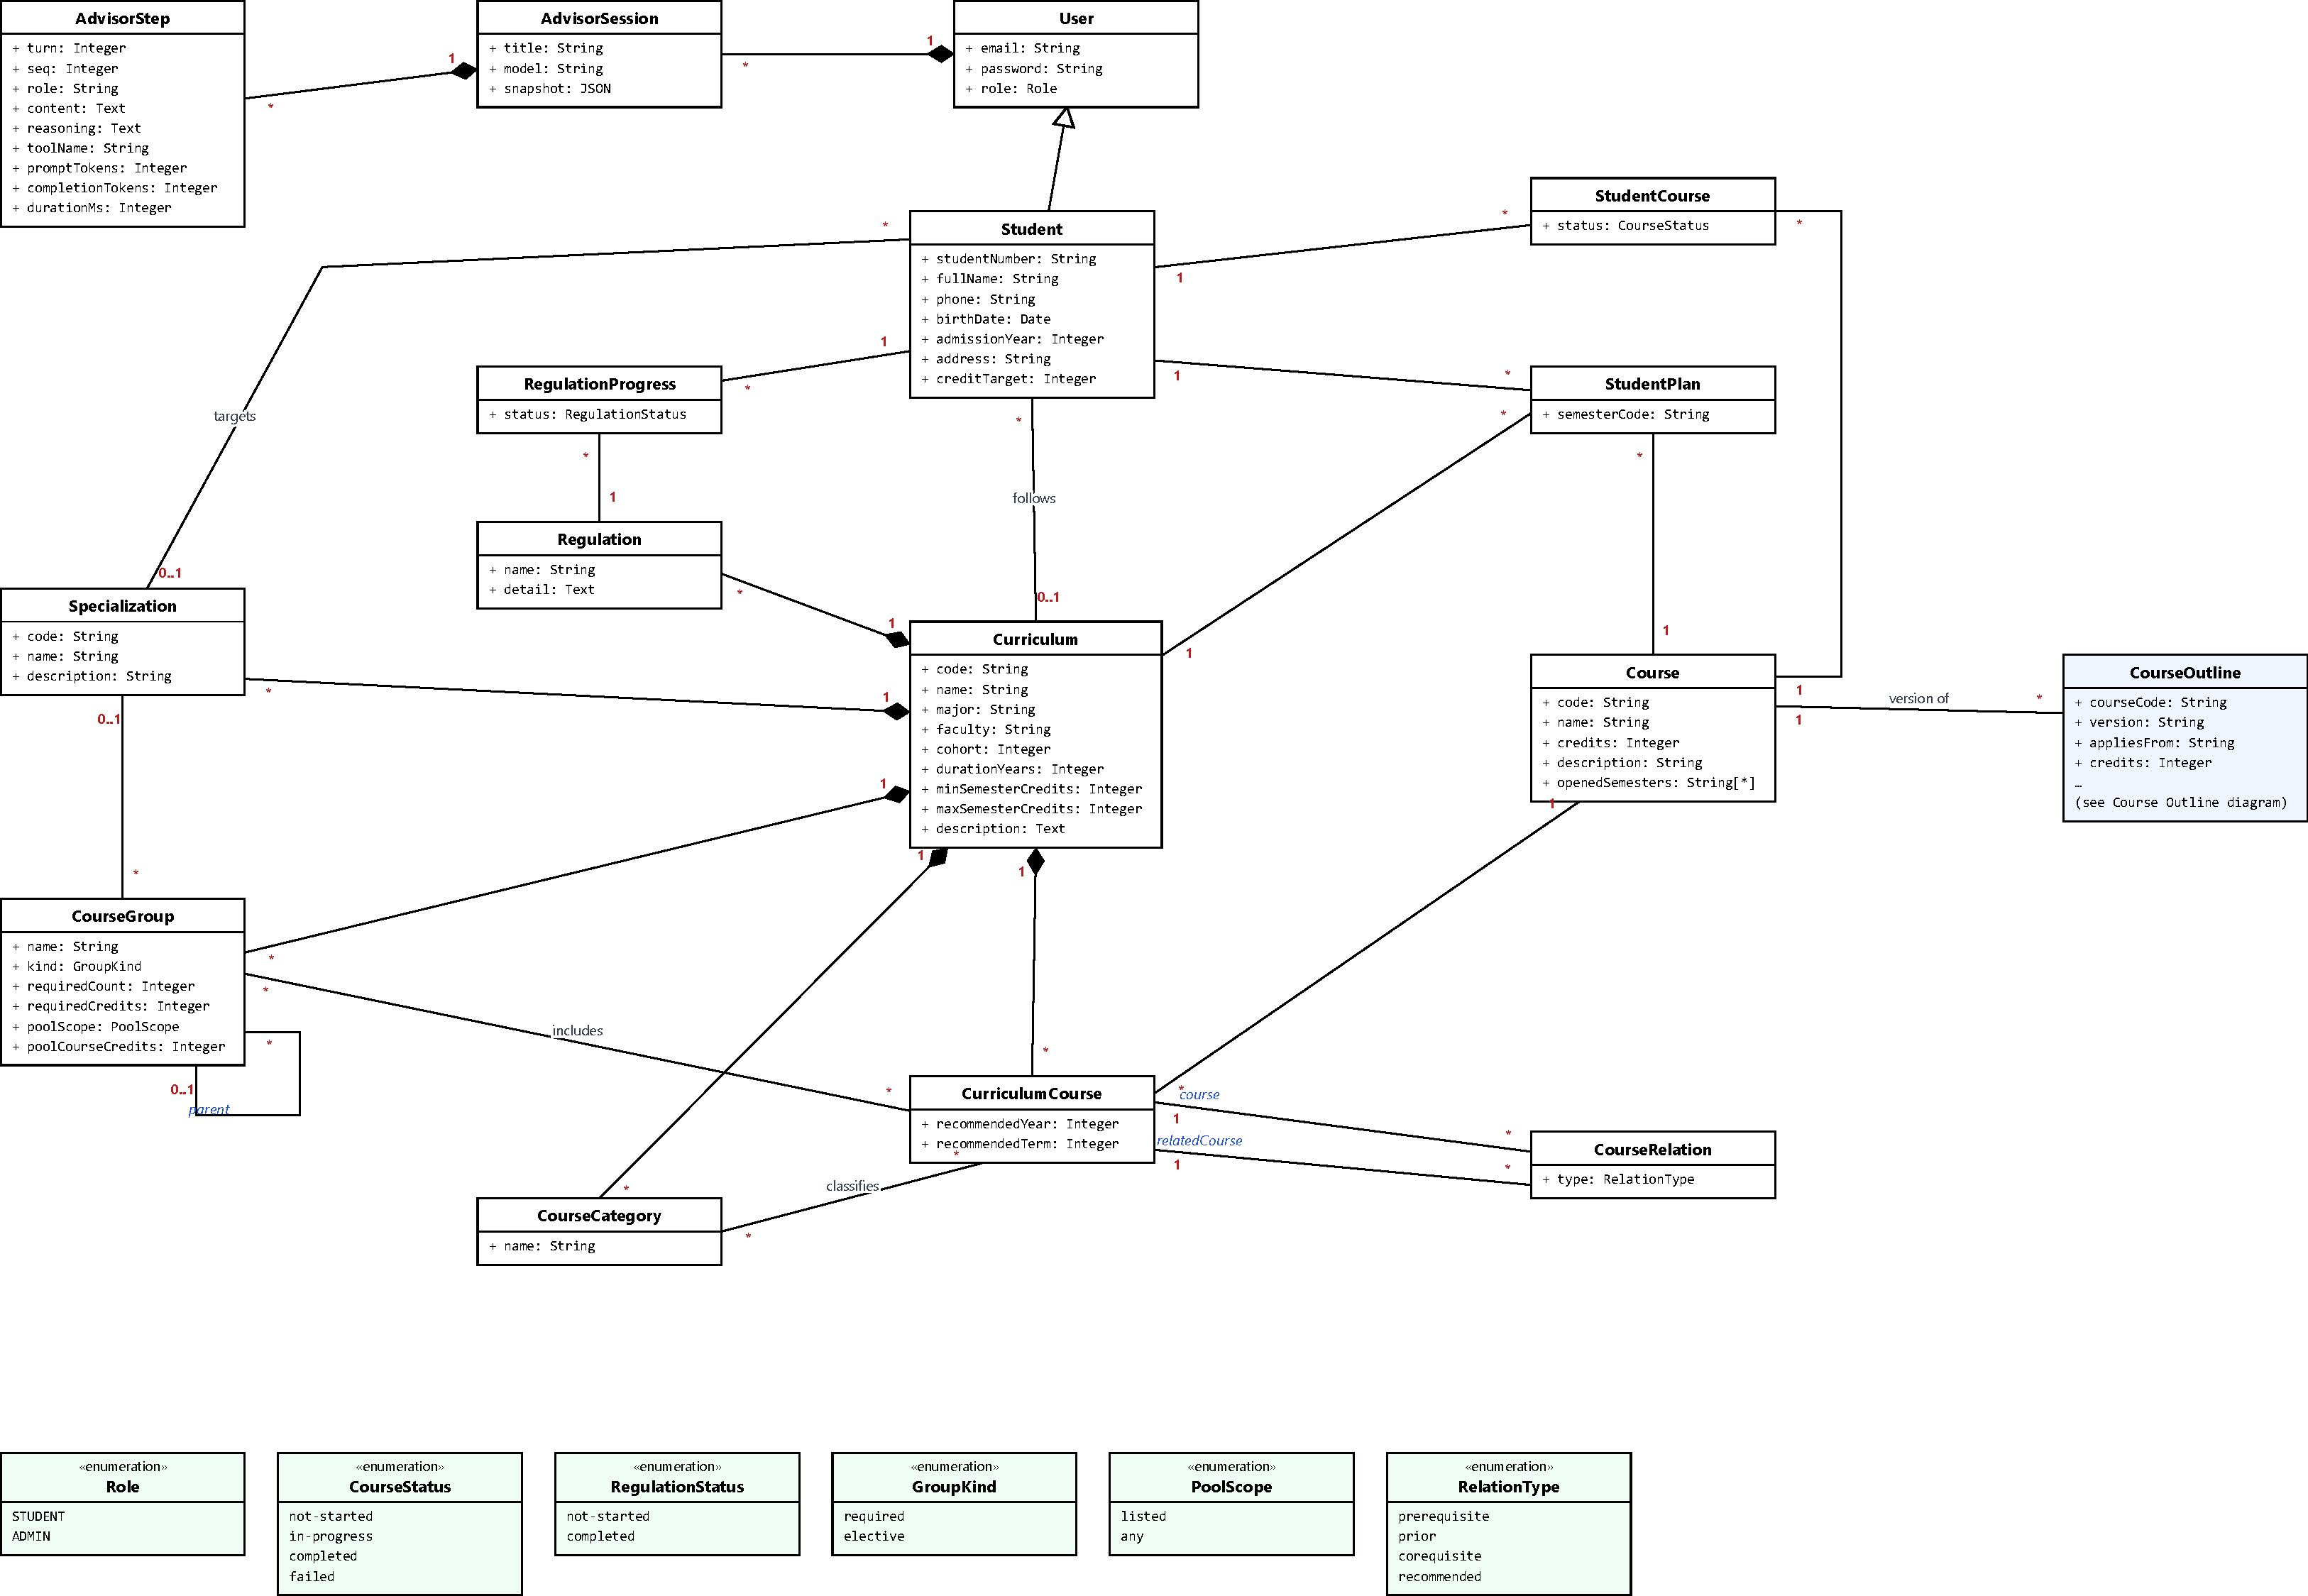
\includegraphics[width=\linewidth,height=0.9\textheight,keepaspectratio]{image/class-diagram.pdf}
        \caption{System overview class diagram}
        \label{fig:class-diagram}
    \end{figure}
\end{landscape}
\restoregeometry
\setlength{\headheight}{40pt} % restoregeometry resets the header height set in h_and_d.tex

% Class diagram on its own landscape page, without header and footer
\newgeometry{margin=1.2cm}
\begin{landscape}
    \thispagestyle{empty}
    \begin{figure}[p]
        \centering
        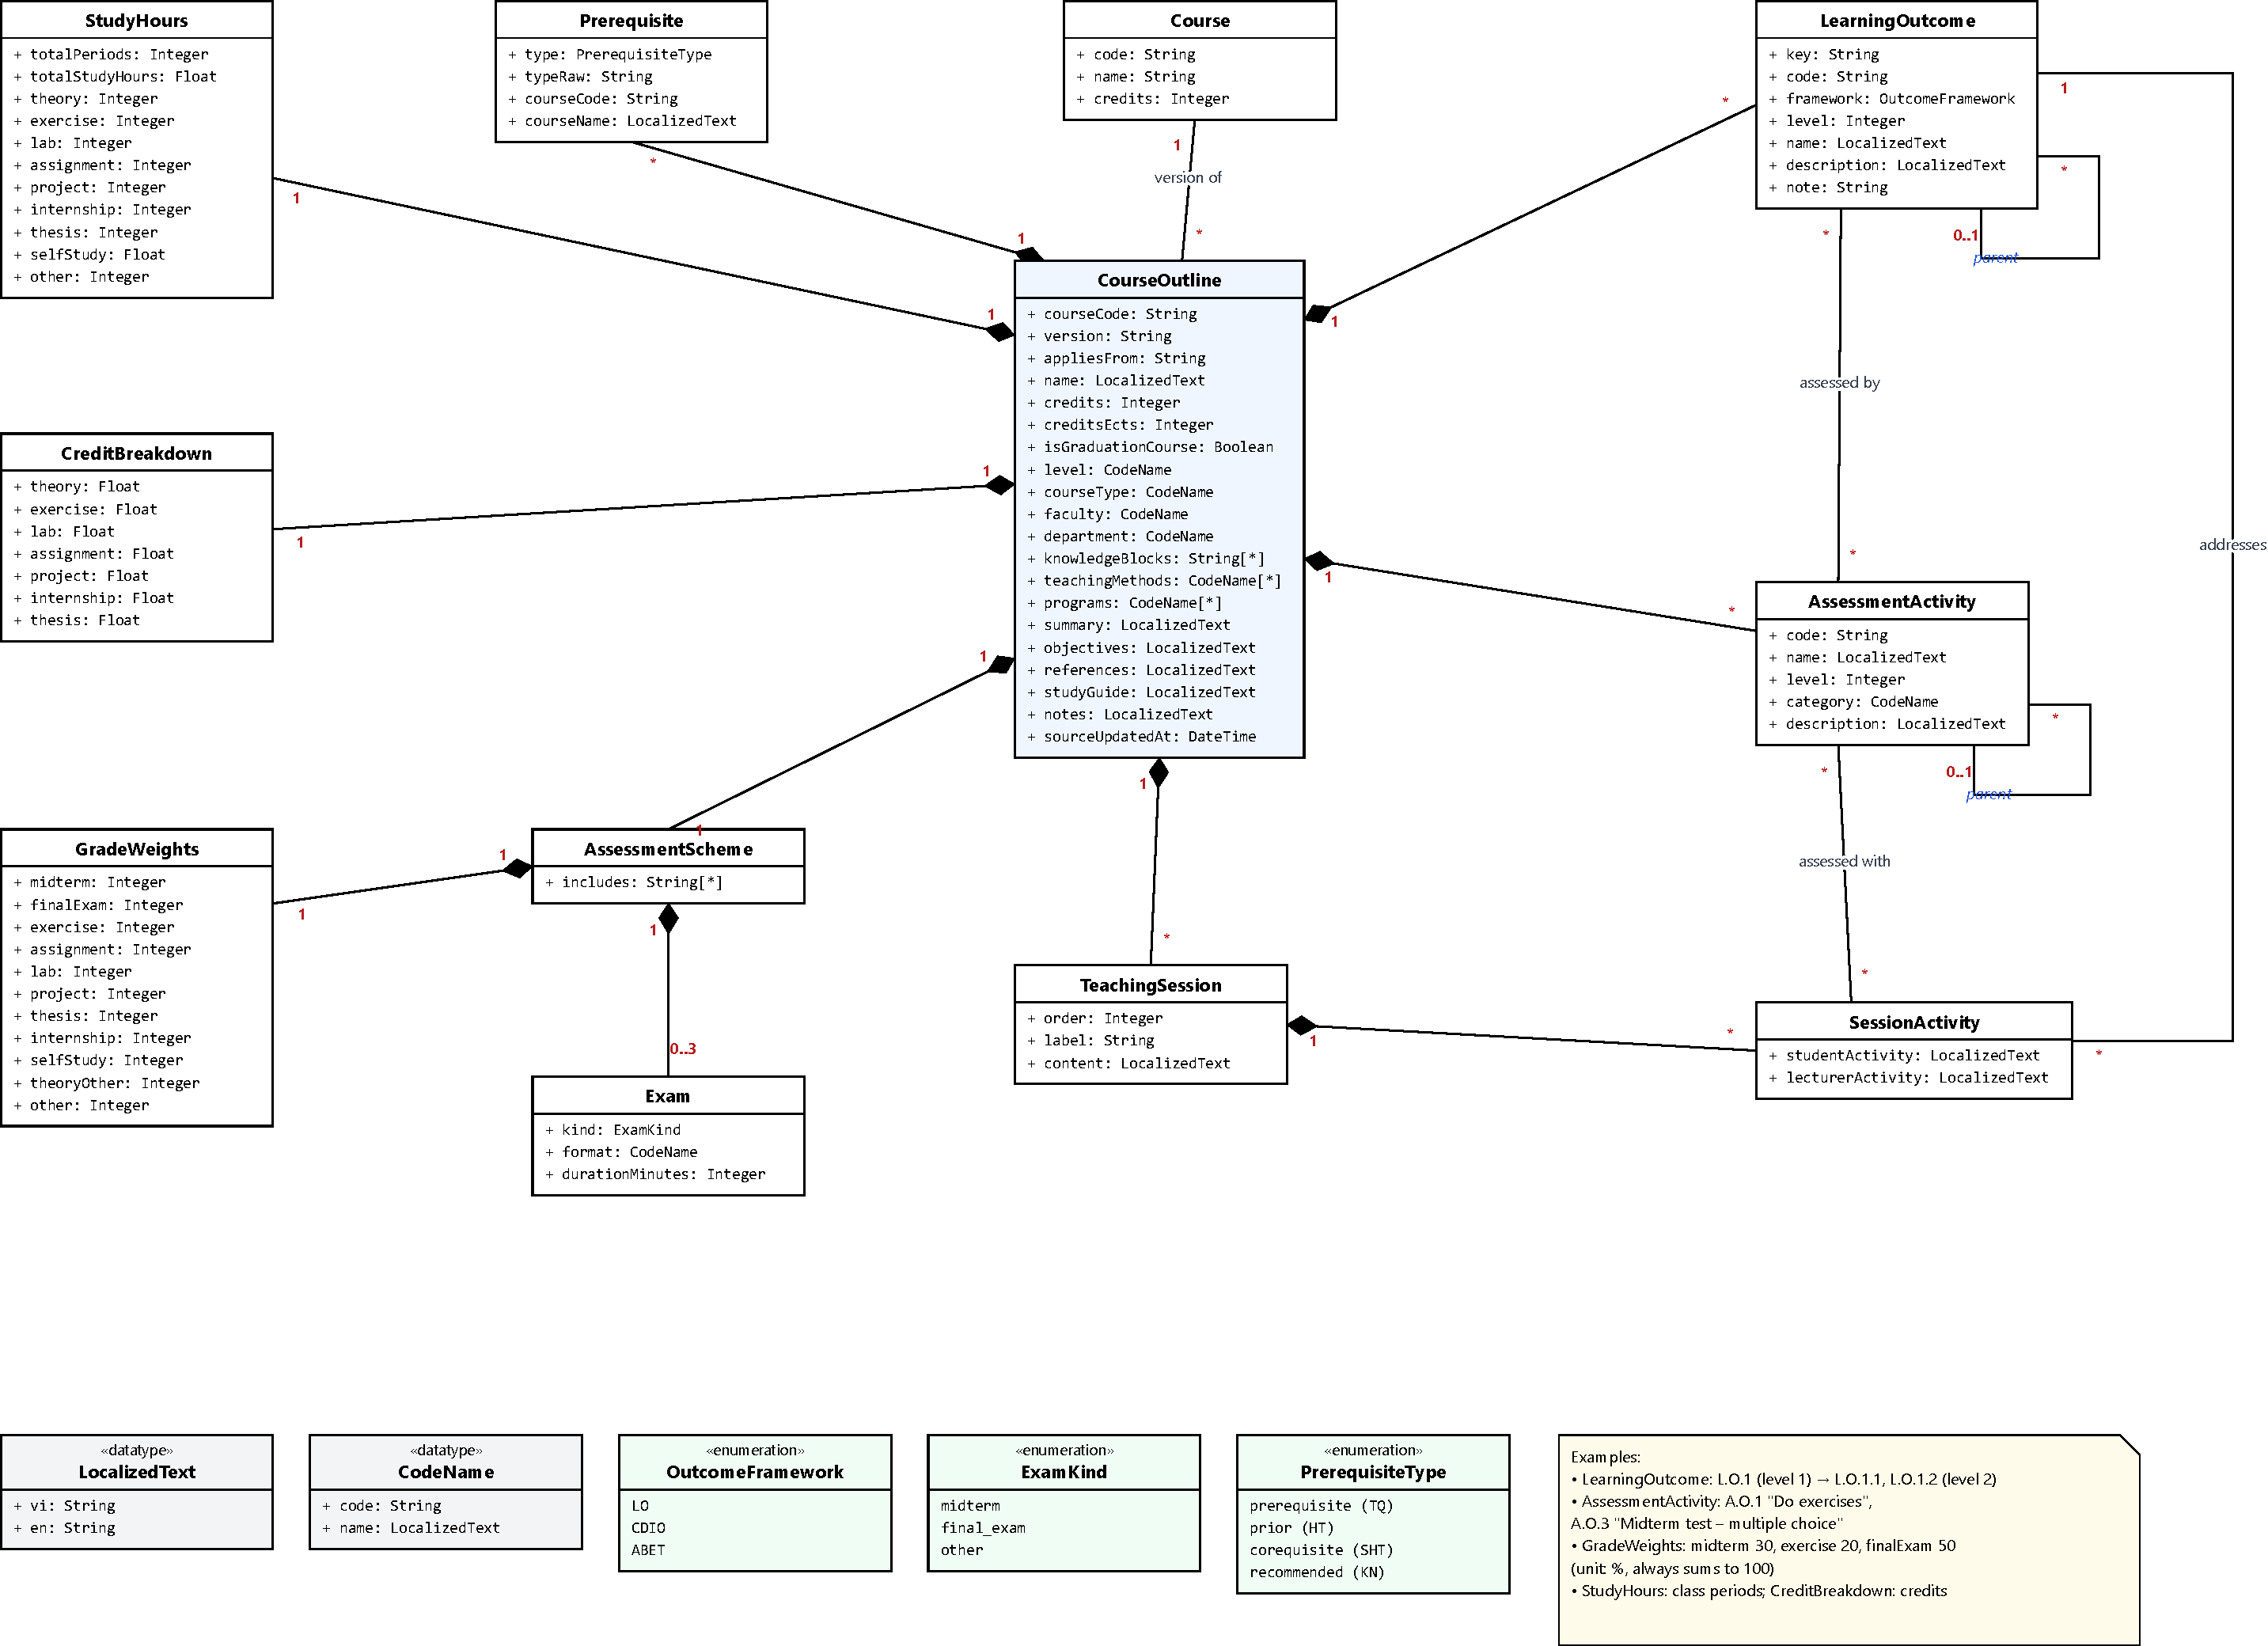
\includegraphics[width=\linewidth,height=0.9\textheight,keepaspectratio]{image/class-diagram-course-outline.pdf}
        \caption{Course outline class diagram}
        \label{fig:class-diagram-course-outline}
    \end{figure}
\end{landscape}
\restoregeometry
\setlength{\headheight}{40pt} % restoregeometry resets the header height set in h_and_d.tex
